%\title{beavtex}
\documentclass[1.5,11pt]{beavtex}
\usepackage{graphicx}
\usepackage{svg}
\usepackage{epigraph}
% \setlength\epigraphwidth{.8\textwidth}
% \setlength\epigraphrule{0pt}
\usepackage{rotating} %Package added to allow the rotation of figures and chart on a page, {sidewaysfigure} command
\usepackage{tablefootnote} %Packaged added to allow footnotes in the tabular environment, use \tablefootnote command
\usepackage{hyperref}
\hypersetup{
    colorlinks=true,
    linkcolor=blue,
    filecolor=magenta,      
    urlcolor=cyan,
}
\usepackage{lmodern}
\usepackage{minted, xcolor}
\usemintedstyle{monokai}
\definecolor{bg}{HTML}{282828}
\usepackage{titlesec}
\usepackage{enumitem}
\usepackage{varwidth}
\usepackage{outline}
\usepackage{amsmath}
\usepackage{amssymb}
\usepackage{tasks}
\usepackage{apacite}

% fancy quotes
\definecolor{quotemark}{gray}{0.7}
\makeatletter
\def\fquote{%
    \@ifnextchar[{\fquote@i}{\fquote@i[]}%]
           }%
\def\fquote@i[#1]{%
    \def\tempa{#1}%
    \@ifnextchar[{\fquote@ii}{\fquote@ii[]}%]
                 }%
\def\fquote@ii[#1]{%
    \def\tempb{#1}%
    \@ifnextchar[{\fquote@iii}{\fquote@iii[]}%]
                      }%
\def\fquote@iii[#1]{%
    \def\tempc{#1}%
    \vspace{1em}%
    \noindent%
    \begin{list}{}{%
         \setlength{\leftmargin}{0.1\textwidth}%
         \setlength{\rightmargin}{0.1\textwidth}%
                  }%
         \item[]%
         \begin{picture}(0,0)%
         \put(-15,-5){\makebox(0,0){\scalebox{3}{\textcolor{quotemark}{``}}}}%
         \end{picture}%
         \begingroup\itshape}%
 %%%%********************************************************************
 \def\endfquote{%
 \endgroup\par%
 \makebox[0pt][l]{%
 \hspace{0.8\textwidth}%
 \begin{picture}(0,0)(0,0)%
 \put(15,15){\makebox(0,0){%
 \scalebox{3}{\color{quotemark}''}}}%
 \end{picture}}%
 \ifx\tempa\empty%
 \else%
    \ifx\tempc\empty%
       \hfill\rule{100pt}{0.5pt}\\\mbox{}\hfill\tempa,\ \emph{\tempb}%
   \else%
       \hfill\rule{100pt}{0.5pt}\\\mbox{}\hfill\tempa,\ \emph{\tempb},\ \tempc%
   \fi\fi\par%
   \vspace{0.5em}%
 \end{list}%
 }%
 \makeatother
 %%%%********************************************************************


\titleformat{\chapter}[display]
  {\normalfont\sffamily\huge\bfseries\color{black}}
  {\chaptertitlename\ \thechapter}{20pt}{\Huge}
\titleformat{\section}
  {\normalfont\sffamily\Large\bfseries\color{black}}
  {\thesection}{1em}{}
\titleformat{\subsection}
  {\normalfont\sffamily\bfseries\color{black}}
  {\thesubsection}{1em}{}

\allsectionsfont{\sffamily}
\fontfamily{lmss}\selectfont
\hypersetup{
    colorlinks=true,
    linkcolor=blue,
    filecolor=magenta,      
    urlcolor=cyan,
    citecolor=cyan,
}

\title{\fontfamily{lmss}\selectfont Journey to the Center of GW170817 \\ Bayesian Parameter Estimation of Outflows from \\ Binary Neutron Star Mergers}
\author{Isabel J. Rodriguez}
\degree{Master of Science}
\doctype{Thesis}
\department{Physics}
\depttype{Department}
\depthead{Head}
\major{Physics}
\advisor{Davide Lazzati}
\submitdate{February 26, 2021}
\commencementyear{2021}


\abstract{\fontfamily{lmss}\selectfont The discovery of GW170817 provided the first empirical evidence that merging binary neutron star systems are both progenitors of short gamma-ray bursts, as well as the primary sites of the nucleosynthetic rapid-neutron capture process. Initially detected as gravitational wave (GW) and gamma-ray burst (GRB) triggers, GW170817 was well-localized and follow-up observations detected a kilonova along with the GRB afterglow. Gamma-ray burst afterglows encode information about jet geometry and the environments in which the relativistic jets propagated. However, the information we can garner is limited to regions that are transparent to radiation---meaning it cannot directly give us information about the central engine, the properties of the jet at injection, or tell us how that jet acquires its structure. By using Bayesian parameter estimation analysis to connect astrophysical data with numerical models, we can begin to constrain the properties of these unobservable regions and improve our understandings of short GRBs and neutron star matter. In this work, we performed two separate analyses using {\fontfamily{qcr}\selectfont emcee}, a Python implementation of the Markov Chain Monte Carlo sampling method. We first constrained jet, environment, and observer parameters of a GRB afterglow resulting from an off-axis structured jet. We then used a subset of those results as data in our second analysis to constrain properties of the central engine, neutron star ejecta, and the jet at injection using an outflow model that simulates baryon-loaded wind and jet interactions. In total we were able to constrain 17 parameters, the largest parameter space so far explored using structured jet outflow and afterglow models. We anticipate that with future joint GW-GRB observations of binary neutron star merger events, similar techniques can be used to further probe the nature of neutron star matter, and by extension a neutron star's equation of state.}

%-------------------------ACKNOWLEDGEMENTS-----------------------

\acknowledgements{There are many people who have helped carry me through this journey and to whom I would like to extend my gratitude. I would first like to thank the members of my graduate committee: my major advisor Dr. Davide Lazzati (Physics), my minor advisor Dr. Robert Thompson (Ethnic Studies), as well as Dr. Xavier Siemens and Dr. Cari Maes. 

To the Oregon NASA Space Grant Consortium, especially Catherine Lanier and Randall Milstein for their advocacy and mentorship. I would like to thank Dr. Natchee Brand and the faculty of the Ethnic Studies department for providing me with a second academic home, Terrance Harris and the Black Cultural Center, Dr. Marilyn Mackiewicz, 3D DAM Diverse Dance, BGSA, CoSMAC, and the work of CGE and Disarm OSU.

To the communities I've found in virtual spaces. From \#VanguardSTEM, to \#BlackinAstro and \#BlackinPhysics, to the networks of informal coworking groups that have helped to keep me grounded while working from home during this global crisis. 

To the Black women who have mentored and inspired me: Dr. Tonia Venters who has provided me with unfailing support and encouragement over the years, Dr. Jedidah Isler who reminded me that I had everything I needed to get this done, Dr. Danielle N. Lee from whom I learned the importance of space, place, and time, and Dr. Chanda Prescod-Weinstein for reminding me that you can do both while being unapologetically Black and queer.

Last but not least, I would like to thank my family, my partner Erin, the friends who have been cheering from day one, as well as my undergraduate mentors---Dr. Suzanne Estes, Dr. Mark Weislogel, and Dr. Erik S\'{a}nchez---who believed in me enough to support my decision to pursue graduate studies.

\vspace{0.5cm}
\textit{–IJR}
}
%-------------------------DEDICATION-----------------------------

\dedication{To the trailblazers that cleared a path, to the ones pushing up from the ashes, \\ and to those who found a different way.
\\ \textit{“You are the dreamer, and the dream.”}
\\ –Star Trek: Deep Space Nine

\vspace{2cm}}

\preface{This thesis, and the work therein, was completed on the traditional territories of the Ampinefu Band of the Kalapuya peoples (Corvallis, Oregon), as well as on the traditional territories of the Duwamish and Salish peoples (Seattle, Washington). Oregon State University is a land grant institution that benefits from the dispossession of land from multiple tribal nations including the Klamath and Kalapuya peoples, the Coast tribes of Oregon, and the Western Shoshone bands. The Ampinefu Band of the Kalapuya, on whose land OSU currently occupies, were forcibly removed from their ancestral homelands to reservations located in Western Oregon; they are today members of the Confederated Tribes of Grand Ronde Community of Oregon, and the Confederated Tribes of the Siletz Indians. Despite having raised millions from this land grab, Oregon State University to this day does not offer free tuition for its Indigenous students, nor has it meaningfully addressed the calls to action put forth this past summer by the Ethnic Studies department, which is the only department on campus comprised almost entirely by Indigenous faculty and faculty of color. The author stands in solidarity with Indigenous struggles for the reclamation of sovereignty, stewardship of natural resources, and collective liberation.}

\begin{document}
\maketitle
\mainmatter

%-------------------------1. INTRODUCTION---------------------------

\chapter{\fontfamily{lmss}\selectfont Introduction} \label{ch:Intro}
 \begin{fquote}[R. Lawton][Space, Place and Time][]Where is it? Why is it there? What follows from it being there?
\end{fquote}
% \epigraph{Space, place and time matter.}{Danielle N. Lee}

%-------------------------1.1 BNS detection---------------------------

\section{A Joint Detection} \label{ch:Intro sec:joint detection}

On the 17th of August 2017, two gravitational wave facilities in the US and a third in Italy---collectively referred to as Advanced LIGO-Virgo\footnote{\fontfamily{lmss}\selectfont LIGO is the  Laser Interferometer Gravitational Wave Observatory with two facilities in the US located in Hanford, Washington and Livingston, Louisiana. The Virgo interferometer is located in Santo Stefano a Macerata, Italy. Together, they comprise the LIGO-Virgo collaboration. A new detector, KAGRA (Kamioka Gravitational Wave Detector; Aso et al. 2013), located in  Gifu, Japan will be joining the network no later than 2022. Gravitational wave interferometry and its significance will be discussed in Chapter \ref{ch:Astro theory sec:GWs}.}---detected the chirp of a gravitational wave signal\footnote{\fontfamily{lmss}\selectfont The LIGO detectors rely on data from Virgo in order to triangulate the gravitational wave signals, in addition to placing better estimates on source properties. As shown in Figure \ref{fig:LIGO-Virgo}, the gravitational wave signal was clear in the LIGO Hanford and Livingston data but not visible in the Virgo data due to the lower source horizon and direction with respect to Virgo's antenna (Abbott et al. 2017). However, a low signal was detected by Virgo which allowed for improved sky localization (though it was too low to contribute to source estimation).} (Abbott et al. 2017). That signature chirp, shown in Figure \ref{fig:LIGO-Virgo}, was indicative of the collision of two compact objects approximately 40 megaparsecs ($\sim$ 130 million lightyears) away.  Less than 2 seconds later\footnote{\fontfamily{lmss}\selectfont Approximately 1.74 seconds later (Lazzati et al. 2020, Goldstein et al. 2017, Zhang et al. 2018).}, NASA's Fermi Gamma-ray Space Telescope (Goldstein et al. 2017) and the European Space Agency's INTEGRAL\footnote{The INTErnational Gamma-Ray Astrophysics Laboratory.} (Savchenko et al. 2017) space telescopes detected a flash of gamma-rays (Fig. \ref{fig:time-delay}, bottom).

Observational data from astrophysical events comes to us from four unique sources, or messengers. Light is the messenger that we are most familiar with. Ancient astronomers, the world's first being from among the Aboriginal and Torres Strait Islander people, studied the patterns made in the sky by the Sun, Moon, and stars to develop sophisticated systems of navigation and timekeeping. Today we have tools that expand our ability to observe beyond the visible spectrum, including everything from radio waves to gamma-rays (we use the umbrella term \textit{electromagnetic radiation} to refer to this broad range of wavelengths). Other messengers include the elusive subatomic neutrino particle, cosmic rays (high-energy electrons, neutrons, and atomic nuclei) and most recently, ripples in the fabric of space-time called \textit{gravitational waves}. Multimessenger astronomy, then, is the case in which a single cosmic event yields observations from two or more of the above sources. An example close to home is the detection of both electromagnetic radiation and cosmic rays emanating from the Sun, but one of the most well-cited examples in astronomy is the detection of neutrinos followed by electromagnetic radiation from the supernova detected in 1987 (designated SN1987A) that occurred in our Milky Way's dwarf satellite galaxy, the Large Magellanic Cloud (e.g., Alexeyev et al. 1988, Hirata et. al 1987, Nisenson et al. 1987).

\pagebreak[4]
\begin{figure}[h!]
  \centering
%   \def\svgscale{0.5}
  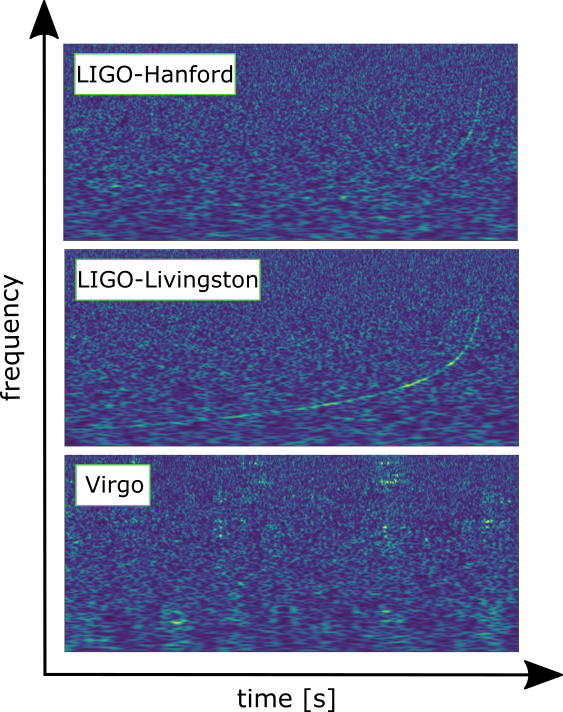
\includegraphics[scale=0.50]{images/ch1/GW-observations.png}
  \caption{\fontfamily{lmss}\selectfont   Advanced LIGO-Virgo observations of GW170817. The gravitational wave signal was clear in the LIGO Hanford and Livingston data but not visible in the Virgo data due to the lower source horizon and direction with respect to Virgo's antenna. Image credit: LIGO-Virgo.}
  \label{fig:LIGO-Virgo}
\end{figure}


Up until 2017, LIGO detectors had been triggered by collisions consistent with that of binary black hole mergers. The detections made on August 17th, however, differed from the usual black hole detections in two important ways. ``Chirps" made by colliding black holes only last for a few seconds---whereas the one LIGO detected lasted nearly one hundred seconds. At about 1.1 and 1.6 times the mass of the sun, LIGO's mass estimates of the compact objects were too low to be black holes (at the time, objects were clocking in anywhere between 7 and 50 solar masses; Abbott et al. 2019). Rather, they were in the range of neutron stars, cores of dead stars about 20 kilometers (12 miles) in diameter. This evidence, together with the near-instantaneous flash of gamma-rays from the same patch of sky, pointed to the strong possibility that the first-ever binary neutron star merger had been detected---and it marked the first time that gravitational radiation was detected jointly with electromagnetic radiation. The gravitational wave component was designated GW170817, while the gamma-ray component was designated GRB170817A. While this was a joint detection, the event is typically referred to only as GW170817. 

This joint-detection alerted the astronomical community to send dozens of ground and space telescopes around the world to point towards that same patch of sky in an attempt to catch a glimpse of the remnants of that explosion and its fading glow. Between the three gravitational wave detectors, and two gamma-ray space telescope detections, the patch of sky containing the origin of the signals was well-localized\footnote{\fontfamily{lmss}\selectfont In April 2019, a potential second neutron star merger was detected. However, it had only been detected by one of the LIGO facilities as the second had been off-line, and the Virgo detector was not triggered. This left astronomers with a poorly-constrained (i.e., very large) patch of sky that did not turn up an electromagnetic component during telescope follow-ups. Because this component was not found, the true nature of GW190425 is unknown (Abbott et al. 2020).}. The three-component follow-up campaign for GW170817 detected an astronomical transient, designated AT2017gfo, in the galaxy NGC4993, eleven hours after the joint detection (Coulter et al. 2017). AT2017gfo was interpreted as the presence of a kilonova explosion (Perego et al. 2017), thus confirming the first ever detection of colliding neutron stars.

A story was slowly beginning to take shape: Approximately 130 million years ago in the galaxy NGC4993, two neutron stars whose once-stable orbit began to decay started to inspiral. In their final moments, the neutron stars collided and merged, prompting one of the most powerful explosions in the universe---one that was serendipitously pointing in our general direction. Follow-up observational campaigns have given us a nearly complete overview of a binary neutron star merger event, but what do the details of the story look like?

\begin{figure}[htbp]
  \centering
%   \def\svgscale{0.5}
  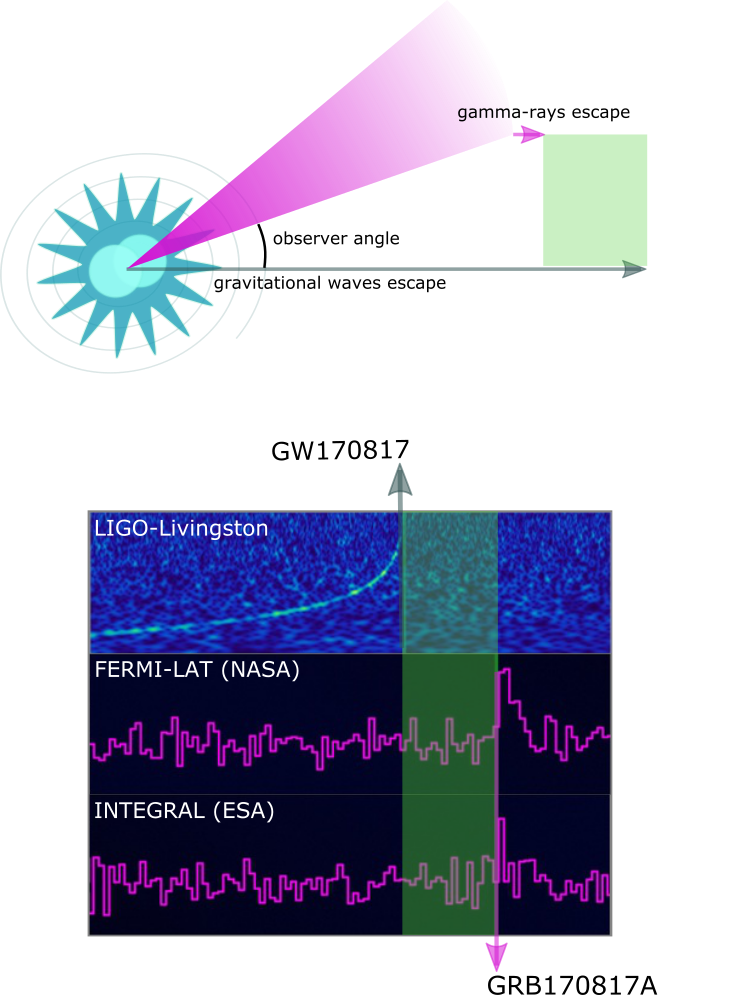
\includegraphics[scale=0.55]{images/ch1/time-delay-2.png}
  \caption{\fontfamily{lmss}\selectfont \textbf{Top:} A visual schematic of what is thought to be the cause of the the 1.74 s delay (highlighted in green) between the gravitational wave and gamma-ray sources. The gamma-rays (magenta), inclined at the observer angle, must first ``break through" an optically thick region before they can flow freely (shown as a color gradient), whereas the gravitational waves (grey) propagated unimpeded. \textbf{Bottom:} The same delay visualized in the data from LIGO-Livingston and the FERMI and INTEGRAL space satellites. The time delay between the detections of GW170817 and GRB170817A is highlighted in green. Image credit: LIGO, NASA, ESA.}
  \label{fig:time-delay}
\end{figure}
% \pagebreak

\clearpage
\subsection{The anatomy of a binary neutron star merger.}
\label{ch:Intro ssec: a BNS merger}

\begin{figure}[ht!]
  \centering
%   \def\svgscale{0.5}
  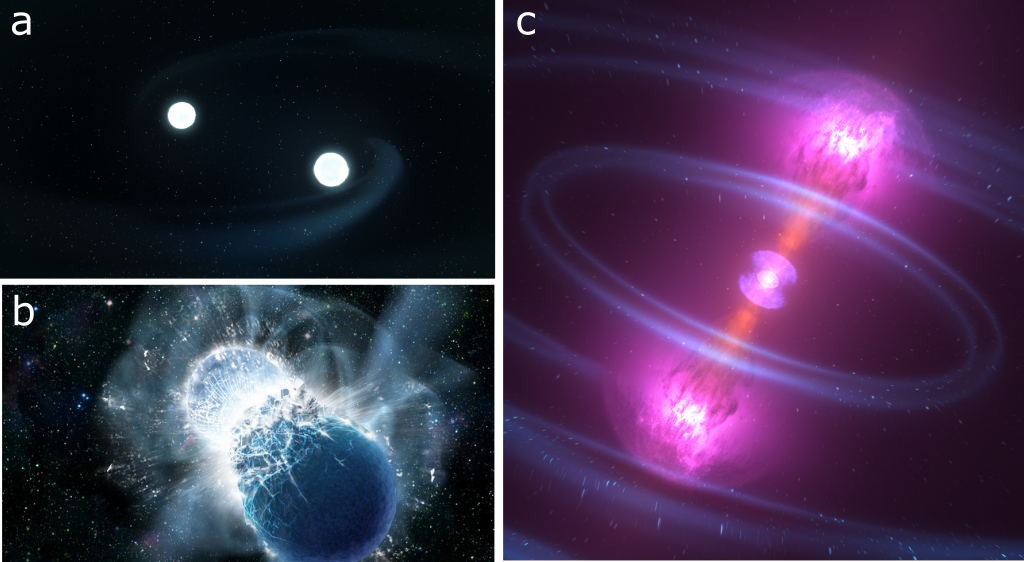
\includegraphics[scale=0.40]{images/ch1/merger_stills.png}
  \caption{\fontfamily{lmss}\selectfont Stills from artists' renderings of a binary neutron star merger event, beginning with the final inspiral (a) and ending in the explosion which produces a kilonova and gamma-ray burst (c). A full video can be found on \href{https://www.youtube.com/watch?v=x_Akn8fUBeQ}{NASA Goddard's} YouTube channel. Image credit: NASA.}
  \label{fig:NS merger}
\end{figure}

\textit{Gravitational radiation–} Figure \ref{fig:NS merger} shows a breakdown of a binary neutron star merger and its aftermath, and Figure \ref{fig: multiwavelength} shows the timeline of the multimessenger and multiwavelength observations of GW170817. Gravitational energy was radiated in the form of gravitational waves during the final minutes of the inspiral of the two neutron stars. This signal increased in amplitude and frequency until it reached the threshold to be detected by Advanced LIGO-Virgo as a chirp (Radice et al. 2020). At or before the moment of coalescence, neutron-rich material became unbound from the neutron stars, creating a field of debris\footnote{\fontfamily{lmss}\selectfont There are two ways to create ejecta: tidal effects and compression-based events. To determine which depends on the neutron star's equation of state, however no direct evidence of tidal interactions has been uncovered (Metzger 2019, De et al. 2018).}. 

\textit{Kilonova–} The initial explosion accelerated the surrounding debris field in a kilonova (e.g., Radice et al. 2020, Perego et al. 2017, Horowitz 2019, Metzger 2019). An image of the kilonova taken in optical by the Hubble Space Telescope is shown in Figure \ref{fig: Hubble image}. Observations made of the astronomical transient AT2017gfo, interpreted to be the kilonova associated with GW170817, revealed a blackbody-like (thermal) spectrum in optical, ultraviolet (UV) and infrared (IR) wavelengths. In less than 24 hours it peaked and faded rapidly in the optical/UV wavelengths (Nicholl et al. 2017), and it peaked after several days in IR (Chornock et al. 2017). The peaks were separated into two distinct components: the blue component for the optical/UV and the red component for IR---these were observations that pointed to the fact that the collision ejecta was dynamic with large velocities (disfavoring the idea that the ejecta was a disk wind created by black hole-neutron star mergers, Nicholl et al. 2017), containing multiple components and challenging previous theoretical models of kilonova (e.g., Perego et al. 2017, Cowperthwaite et al. 2017). 


\begin{figure}[htbp!]
  \centering
%   \def\svgscale{0.5}
  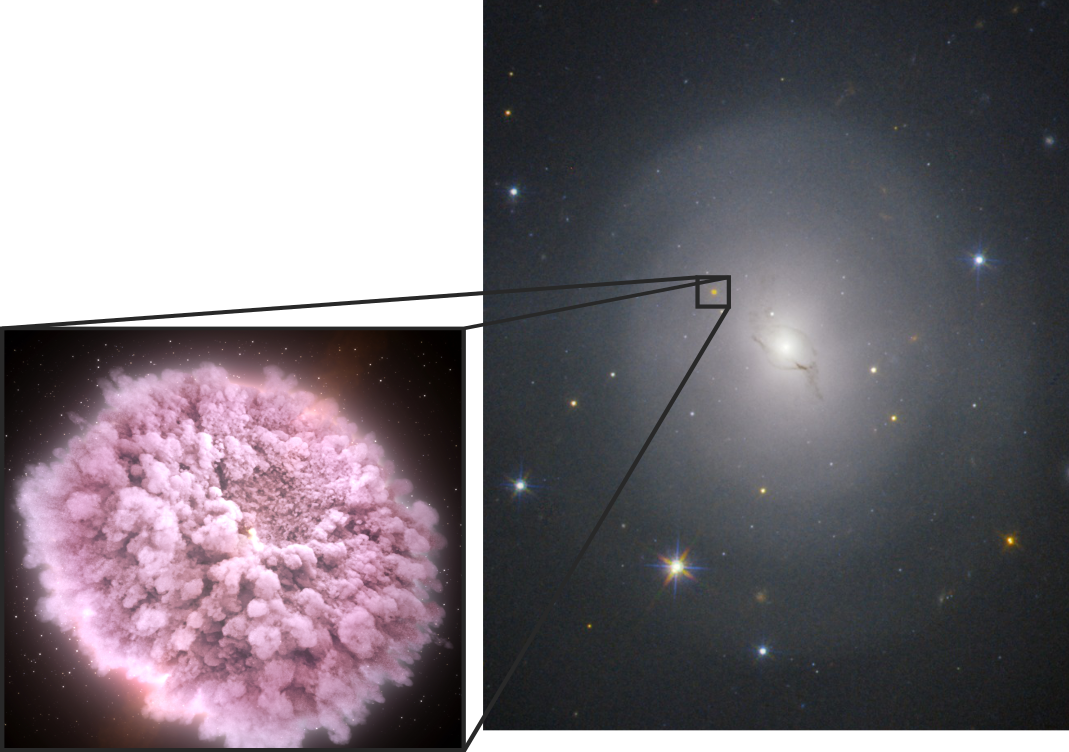
\includegraphics[scale=0.35]{images/ch1/Hubble-kn-square.png}
  \caption{\fontfamily{lmss}\selectfont  \textbf{Right:} Hubble image of the kilonova (marked with a grey square) associated with GW170817 located in its host galaxy, NGC4993. \textbf{Left:} Artist rendition of the red component of a kilonova explosion. Image credit: NASA.}
  \label{fig: Hubble image}
\end{figure}


\textit{Relativistic jet–} The explosion also prompted the launch of a jet traveling at nearly the speed of light, a jet that was bright in gamma-rays---a gamma ray burst. The burst lasted less than 2 seconds, placing it in the category of short gamma-ray bursts (these, and gamma-ray bursts more generally, will be discussed in Chapter \ref{ch:Astro theory sec:GRBs}). The gamma-ray emission was dimmer than expected, and computational modeling determined this was likely due to the fact that we viewed the jet off-axis (i.e., at an angle; Fong et al. 2019, Alexander et al. 2018, Lazzati et al. 2018). It was through the analysis of afterglow observations with the VLA (Very Large Array; Mooley et al. 2018), and supported by previous numerical modeling by Lazzati et al (2017a,b) that the presence of this relativistic jet was revealed.  

\textit{Afterglow–} In addition to the thermal component, a non-thermal component was also observed in radio (Hallinan et al. 2017), X-ray (Troja et al. 2017), and gamma-rays (Radice et al. 2018) roughly 10 days after the initial trigger. It is thought that this component arose after the relativistic jet eventually interacted with the cooler surrounding interstellar medium (ISM), resulting in shockwaves that are characterized as the afterglow. Whereas the gamma-ray burst was dimmer than expected, its afterglow was bright in X-rays (Margutti et al. 2018). As of summer 2020, X-ray emissions had been visible by NASA's Chandra X-ray telescope for 2.5 years (Troja et al. 2020a). This prolonged emission could be due to a number of different factors , including: 1) a Gaussian structured jet, 2) a kilonova afterglow, or 3) a new feature of the GRB afterglow, caused by either an emission component that was previously unaccounted for, unknown relativistic jet dynamics, or changes to the syncrotron emission spectrum (Troja et al. 2020a, Kathirgamaraju et al. 2019). The current Chandra X-ray dataset is insufficient to distinguish between these different scenarios. An observing run of GW170817 carried out from December 09-13, 2020 (Troja et al. 2020b) observed X-rays that were brighter than their previous observations; while analysis is still ongoing, it may indicate that GW170817 left behind either a (long-lived) supramassive or a stable neutron star (see Fig. \ref{fig:BNS-endpoints}; Sarin and Lasky 2020).

\section{Motivation} \label{ch:Intro sec:Motivation}

In 2017, astronomers observed for the first time a source of the most powerful explosion in the universe: the collision of two neutron stars. This cosmic event first triggered a gamma ray bust that was detected by space-based telescopes, followed by a glow that could be detected by space- and ground-based telescopes for weeks (and years!) afterward. What can data from the light we observed tell us about neutron stars, and how can we leverage numerical simulations to help us with this task? By connecting numerical models directly to observational data using statistical methods, we can study the properties of the jet’s afterglow, and explore how that information can be used to constrain properties of the jet, the neutron star debris that were ejected on impact, and by extension, the neutron stars themselves. These properties, or \textit{parameters}  (e.g., jet energy, jet opening angle) are assigned numerical values, and the iterative process of constraining more precise values using numerical optimization techniques is the process of \textit{parameter estimation}. 

There are a number of parameter estimation studies of GW170817 in the literature, some of them using only data from the electromagnetic component, and some taking the multimessenger approach. Some of the things we've learned through the combination of simulations and parameter estimation include: that we viewed the event approximately 15-30 degrees off-axis (e.g., Lazzati et al 2018, Lazzati et al 2017); jet opening angle at injection ($\sim 17.9^{\circ}$; Lazzati et al. 2020); the amount of neutron star debris ejected during the merger event, including the fraction of the neutron star debris that was accelerated into dynamical ejecta ($\sim$ 0.03-0.06 solar masses; e.g., Radice et al. 2018, Radice and Dai 2019, Cowperthwaite et al. 2017) and how much remained as an accretion disk ($\sim$ 0.2 solar masses); constraints on both the tidal deformity and radii of the neutron stars (e.g., De et al. 2018), as well as the neutron star equation of state (e.g., Radice and Dai 2019, Radice et al. 2018); constraints on the orbital eccentricity of GW170817 ($e \leq 0.024$; Lenon et al. 2020) and more generally, the effect eccentricity has on nucleosynthetic yields (e.g., Papenfort et al. 2018). Parameter estimation has also provided supporting evidence that the two neutron stars had comparable masses (Radice and Dai 2019), an inference of the rate of neutron star mergers, as well as the fraction of those that would lead to GW170817-like events\footnote{\fontfamily{lmss}\selectfont According to Beniamini et al (2018), roughly one to ten percent of neutron star mergers, which form at a rate of $\sim 0.02 \mathrm{Gpc}^{−3} \mathrm{yr}^{−1}$ (Ye et al. 2020) would be detectable both in gravitational waves and in gamma rays.} (e.g., Beniamini et al. 2018). 

The research described in this thesis adds to this growing body of work by addressing the following questions: 

\begin{enumerate}
    \item By using multiband observations of the afterglow in combination with a numerical model that simulates the afterglow from an off-axis structured jet, what can we learn about key parameters of the jet, circumburst environment, and inclination associated with GW170817?  
    \item Can we use properties of the structured jet obtained from (1) to constrain intrinsic properties of the jet (its properties before interacting with its environment), neutron star ejecta, and the central engine? 
\end{enumerate}

\begin{figure}[htbp!]
  \centering
  \def\svgscale{0.3}
  \includesvg{images/ch1/multiwavelength_observations.svg}
  \caption{\fontfamily{lmss}\selectfont A timeline of the multimessenger observations of GW170817, GRB170817A, and AT2017gfo. The timeline begins with the LIGO-Virgo gravitational wave detection (top left) and ends with the gamma-ray burst afterglow detections by Chandra and the VLA (bottom right).  Image credit: Hartley (2017).}
  \label{fig: multiwavelength}
\end{figure}
\pagebreak[4]
\clearpage

%-------------------------1.2 This thesis---------------------------
\section{Thesis Overview} \label{ch:Intro sec:Thesis overview}

Computational tools have enabled exciting synergies between observation and theory, allowing us to translate cosmic phenomena into numerical interpretations of physical descriptions that can then be used to inform future observations. In turn, those improved observations may help us distinguish between competing interpretations. Constructing a physical description of gamma ray burst afterglows requires an understanding of stars and their environments, the physics of radiation transport mechanisms, and the kinds of computational techniques that optimize the information we can extract from numerical models and observational data.

To this end the content of this thesis encompasses: 1) current models of stellar evolution, with a focus on binary star systems, their evolutionary endpoints, and the relativistic outflows those endpoints can produce; 2) the theoretical framework behind the probabilistic data analysis used in this work; 3) results of parameter estimations made using a pure Python implementation; 4) a discussion of these results, where to find the code used in this work, as well as open questions and opportunities for improvement. As a final note, this thesis makes a concerted effort to ground scientific advancements in a social-historical context, the (re)telling of which is guided by a Black queer feminist lens\footnote{\fontfamily{lmss}\selectfont Charlene Carruthers defines the Black queer feminist lens as ``a political praxis (practice and theory) based in Black feminist and LGBTQ[IA+] traditions and knowledge, though which people and groups see to bring their full selves into the process of dismantling all systems of oppression." (Carruthers, 2018, p.10). This knowledge descends from theories put forth by, for example, The Combahee River Collective (1977), hooks (1984), Lorde (1984), and Collins (2000), and put into a STEM context by e.g., Malcom et al. (1976), Chambers 2019, and Isler et al. (2021).} that interrogates the dominant science canon. 

%-------------------------2 Theory: The Astrophysics---------------------------
\chapter{Neutron Stars, Gamma-Ray Bursts, and Gravitational Waves} \label{ch:Astro theory}
\begin{fquote}[Chanda Prescod-Weinstein][Are we just making things up?] Everything theoretical physicists do is speculative, and likely wrong, except for the things we get right.
 \end{fquote}

\textit{Overview.–} This chapter serves as a brief primer on stellar evolution, with a focus on high-mass binary star systems, how they lead to high-energy and gravitational wave phenomena like GW170817. 

%-------------------------2.1 A Primer on NSs---------------------------

\section{A Primer On Neutron Stars} \label{ch:Astro theory sec:NS}

In the previous section, I alluded to the fact that neutron stars are the endpoint of a star's life, but this isn't the fate of all stars. To understand neutron stars, as well as other endpoints to stellar evolution that drive interesting astrophysical phenomena, we begin with our current understanding of what a star is and how it evolves.  

\subsection{What is a star?}
\label{ch:Astro theory ssec:what is a star}

Stars are are the most fundamental building blocks of the observable Universe. If the light pollution is low enough\footnote{\fontfamily{lmss}\selectfont Around the globe, pristine dark skies are becoming increasingly hard to find. Light pollution impacts not only the ability of amateur and professional astronomers to observe the night sky, but it also has negative impacts on human health as well as wildlife ecology. In 2015 the Kaibab Paiute Tribe, after years of organizing on their traditional homelands (now known as Northern Arizona), was designated the world's first ``Dark Sky Nation" by the International Dark-Sky Association (IDA; Hunter 2015)---an organization that works to preserve the night sky as a heritage for future generations.}, they are some of the first things we see in the night sky. They are hot, dense, ionized balls of plasma whose equilibrium is characterized by two things: 1) the inward pull of their own self-gravity, combined with the downward gas pressure, that is countered by 2) the outward push of gas pressure and radiation pressure\footnote{\fontfamily{lmss}\selectfont Gas pressure is the combined pressure of the electrons and ions, whereas radiation pressure is produced via nuclear fusion in the star's core. Low-mass stars are dominated by gas pressure, and high-mass stars are dominated by radiation pressure}. Stars produce, in various nucleosynthetic processes not limited to fusion, most of the elements in the periodic table–including the carbon, oxygen, and nitrogen our bodies are made out of. Stars come in an assortment of sizes and the vast majority of the most massive stars are found in pairs (Sana et al. 2012), with some stars forming triple, quadruple, or larger systems.

Given this fact, and given that each galaxy is home to billions of stars, it is likely that there are many binary neutron star systems (also known in the literature as double neutron star, or DNS, systems). Because they are difficult to detect, however, there are currently only 19 known BNS systems in our Galaxy (Zhu and Ashton 2020), the first of which was discovered in 1974 (Hulse and Taylor 1975). In the sections below, I will touch on the different tracks of stellar evolution as well as the evolution of binary star systems.

\subsection{Stellar evolution}
\label{ch:Astro theory ssec:Stellar evo}

\begin{figure}[ht!]
  \centering
%   \def\svgscale{0.5}
  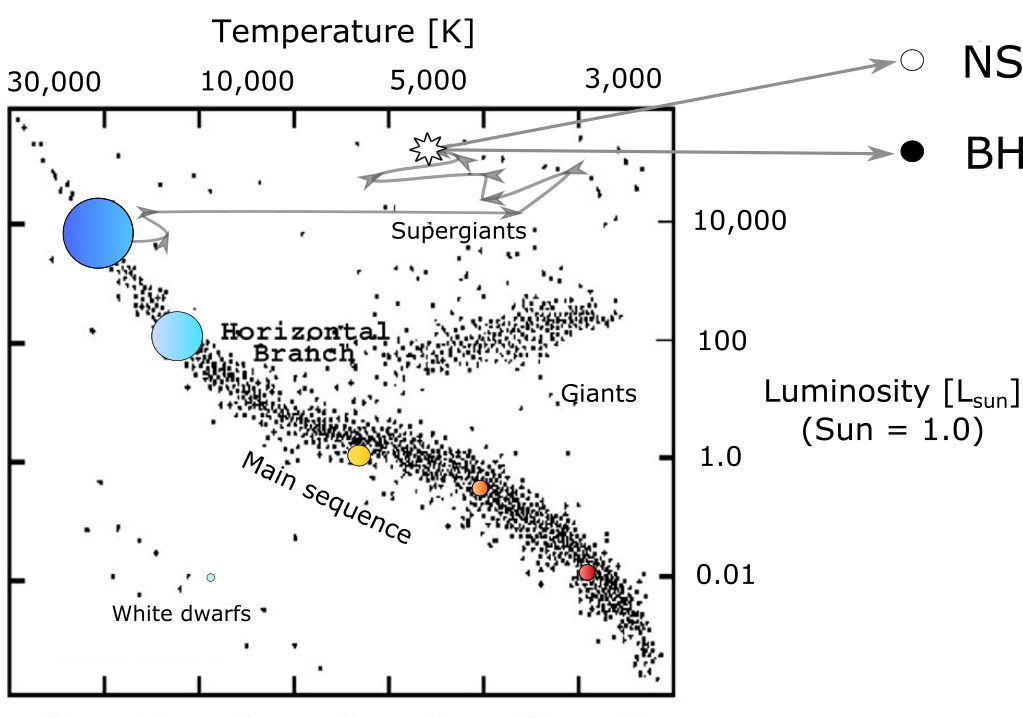
\includegraphics[scale=0.50]{images/ch2/HR-diagram-HM.png}
  \caption{\fontfamily{lmss}\selectfont The Hertzsprung–Russell (HR) diagram, is used to show the relationship between a star's luminosity and effective temperature. Stars that are in the main sequence are in hydrostatic equilibrium, and their post-main sequence (MS) evolution (i.e., their deaths) have different traces depending on their mass at birth. Our Sun is indicated with the yelow circle. Stars above this point on the MS have higher masses, while the stars below have lower masses. The post-main sequence evolution of a high-mass star is traced in grey. Once it has exhausted its fuel, it will explode in a supernova (indicated by the white burst), and depending on the mass of its core become either a neutron star (NS) or a black hole (BH). Image adapted from: NASA.}
  \label{fig:HR-diagram}
\end{figure}

\textit{The fate of a star is mass-dependent.–} The life-cycle of a star is highly dependent on its mass at birth (Fig. \ref{fig:HR-diagram}), because its mass will determine its core temperature which is critical if it is to sustain itself through nuclear fusion. Stars form from clouds of gas that collapse under their own gravity, the metallicity\footnote{\fontfamily{lmss}\selectfont To astronomers, \textit{metal} refers to anything heavier than H and He, the two elements formed in the universe's first nucleosynthetic process---the Big Bang. Note that here, I will be taking the astronomer's convention and referring to most chemical elements by their element symbol (e.g., hydrogen=H, helium=He, carbon=C, oxygen=O, iron=Fe).} of which tells us whether they belong to the first populations of stars (Population III stars), or whether they were formed more recently from the recycled materials of older generations of stars (Populations II \& I, with the latter being the youngest). Because the Sun is our closest star, and therefore our most familiar, astronomers use its measurements as a base unit for comparing other stars in our Universe. The mass of our Sun ($1.9885 \times 10^{30} \, \mathrm{kg}$) is simplified to 1 solar mass (denoted \(M_\odot\)). In traditional models of stellar evolution there are three distinct tracks, where the masses of stars at birth are compared to the solar mass:

\begin{center}
\begin{varwidth}{\textwidth}
\begin{itemize}
    \item Brown dwarfs ($<$ 0.08 \(M_\odot\)) 
    \item Low-mass stars (0.08 \(M_\odot\) $< \ M_{\mathrm{star}$ $<$ 8 \(M_\odot\))
    \item High-mass stars ($>$ 8 \(M_\odot\))
\end{itemize}
\end{varwidth}
\end{center}
 
 There are many technicalities, uncertainties, and challenges involved in our understanding of stellar evolution, and our agreement of the details is not always perfect. Factors that influence a star's evolutionary trajectory include but are not limited to: spin, the presence of one or more companion stars, stellar wind, and metallicity. These are things that are explored in more detail in astronomy and astrophysics textbooks (e.g., Eldridge and Tout 2019, Carroll and Ostlie 2014, Maoz 2006).  Here, I will present a brief summary.
 
\textbf{Brown dwarfs} are considered substellar objects (i.e., \textit{failed stars}) because they contain an insufficient amount of mass---and therefore too low a temperature at their core---to begin the stable fusion of H $\rightarrow$ He (Hayashi and Nakano 1963). Rather, brown dwarfs glow in infrared due to the internal temperatures sustained by the fusion of deuterium into helium, and later lithium burning (Allard and Homeier 2007). Over the course of one hundred million years, brown dwarfs will exhaust their fuel and contract gravitationally, after which they will spend billions of years undergoing radiative cooling and dimming, eventually becoming cold balls of gas. While they may be considered to be failed stars, with masses between about 10 and 100 times that of Jupiter, brown dwarfs provide us with an interesting link between stars and planets.

\textbf{Low- (and intermediate-) mass stars} comprise the majority of all stars, and are able to to ignite and burn H $\rightarrow$ He. It is at this point that we consider a star to be in hydrostatic equilibrium and on the main sequence (Fig. \ref{fig:HR-diagram}). Stars between 0.08 and 0.8 \(M_\odot\) will have internal temperatures too low to fuse He and so will grow to become a red giant, before shedding its outer layers, or \textit{envelope}, as its core shrinks to reveal a helium white dwarf about the size of the Earth (Eldgridge and Tout 2019). 

Stars between 0.8 and 8 \(M_\odot\) will trace slightly different evolutionary paths, though all will form a C-O core and all will grow into a red giant phase, eventually shedding their envelopes as planetary nebulae. Stars on the lower end of the range like our Sun will be unable to burn C leaving behind a carbon-oxygen white dwarf, whereas more massive stars will be able to ignite C and instead leave behind an oxygen-neon white dwarf (Eldridge and Tout, 2019). Like brown dwarfs, there is no fusion taking place within a white dwarf to counterbalance the relentless pull of its gravity, however both are prevented from collapsing due to electron degeneracy pressure (Basri 2000). This has profound implications for the fate of high-mass stars, as we'll see below.

\textit{Electron degeneracy pressure.–} Degeneracy combines two ideas from quantum mechanics: Pauli's exclusion principle and Heisenberg's uncertainty principle (Carroll and Ostlie 2014). These principles state that no more than one electron can occupy each quantum state, and that an electron with a known position will have an uncertain momentum (and vice versa)\footnote{\fontfamily{lmss}\selectfont Technically, these principles apply to all matter. In atoms, no more than two electrons can occupy each orbital, and each electron must have a different quantum state (spin-up and spin-down).}. As the atoms of a gas are squeezed together tightly, their electrons, once able to move freely in their orbitals, are constrained to the lowest energy quantum states. In order to maintain the uncertainty principle, this means that the electrons' momentum (\textit{i.e.}, their speed) increases. The electrons want to push back to occupy different quantum states, but the force of gravity is too strong to rebound. In the dense cores of stars, the lower energy states are filled and ionized (unbound) electrons are forced to occupy very high energy states. The pressure this creates reestablishes hydrostatic equilibrium. There is an upper mass limit for this configuration to remain stable, known as the \textit{Chandrasekhar limit}, and it defines the theoretical limit for the mass of a white dwarf star: 1.4 \(M_\odot\).  

\begin{figure}[h!]
  \centering
%   \def\svgscale{0.5}
  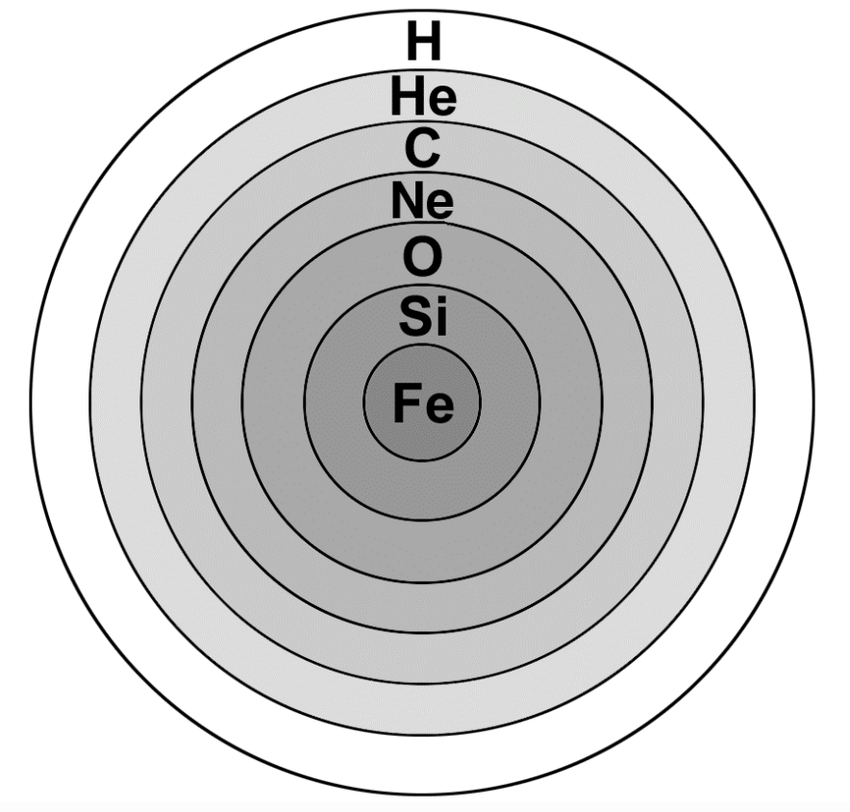
\includegraphics[scale=0.20]{images/ch2/onion-structure.png}
  \caption{\fontfamily{lmss}\selectfont The onion structure of a high-mass star with a Fe core that results from core-shell burning. Once Fe has formed in the core, the star will become unstable and collapse prompting a supernova explosion and producing either a neutron star or a black hole. Image credit: NASA.}
  \label{fig:onion-structure}
\end{figure}

\textbf{High-mass stars} are born with internal temperatures high enough to continue burning where intermediate-mass stars could not, and they do so quickly. Like the evolution of low/intermediate mass stars, evolutionary tracks in high-mass stars will differ depending on mass, as the factor of mass-loss over the course of its life due to stellar winds becomes important. Generally speaking, however, massive stars undergo shell and core burning, generating an onion-like structure until they begin to fuse Fe in their core (see: Fig. \ref{fig:onion-structure}). Because Fe requires energy to fuse, as opposed to creating energy through the fusion process, the core will continue to amass Fe until the Chandrasekhar limit\footnote{\fontfamily{lmss}\selectfont This limit is why neutron stars fall within a range of roughly 1-2 \(M_\odot\), with the average being around 1.35\(M_\odot\). } is exceeded, after which the core begins to collapse and explode in a supernova. We observe these remnants as nebula (Fig. \ref{fig:crab-nebula}). Depending on the mass of the star's core, there are one of two end-points: black holes and neutron stars. 


\subsection{Neutron stars} 
\label{ch:Astro theory ssec:NSs}

\begin{figure}[ht!]
  \centering
%   \def\svgscale{0.5}
  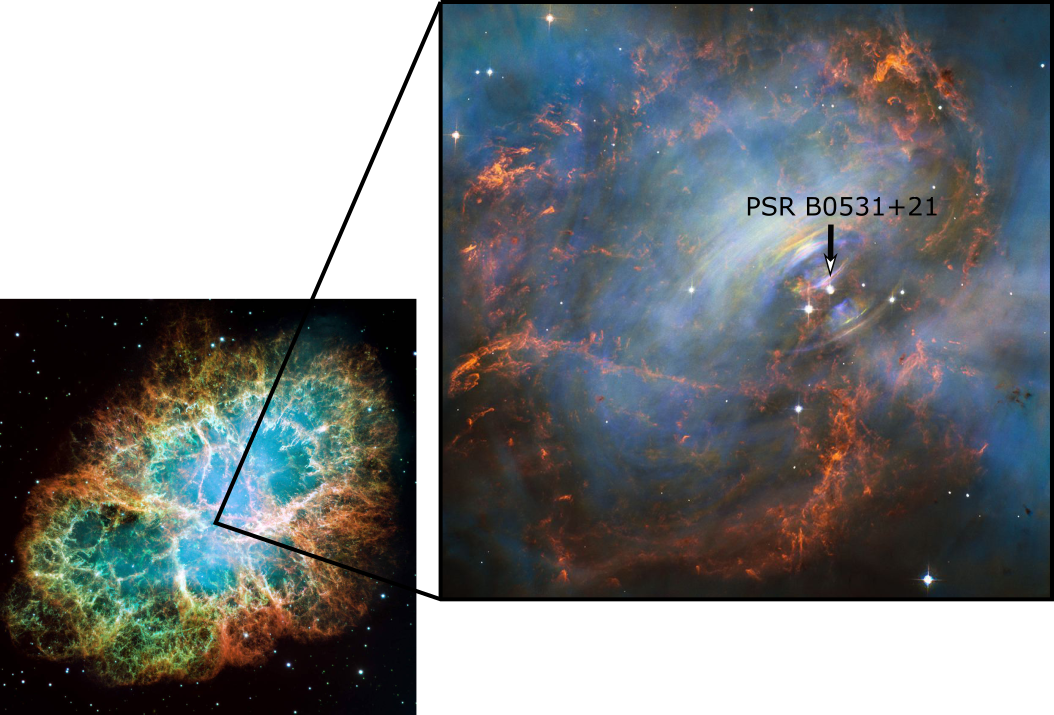
\includegraphics[scale=0.40]{images/ch2/Crab-nebula.png}
  \caption{\fontfamily{lmss}\selectfont At the heart of The Crab Nebula (Messier 1 or M1), a supernova remnant, is the pulsar PSR B0531+21 with a mass comparable to the sun packed into the size of a city. Dynamic wisps and rings expand outward in a pulsar wind. Image credit: NASA, ESA.}
  \label{fig:crab-nebula}
\end{figure}

\textit{Neutron degeneracy pressure.–} Neutron stars are formed when the progenitor star is so massive that the electron degeneracy pressure is overcome and the electrons are squeezed into the protons, creating a dense neutron superfluid that follows the same two quantum principles discussed earlier. As with electron degeneracy pressure, there is also a degeneracy pressure associated with neutrons that are packed too close together. For ``less massive" massive stars, this pressure is enough to halt the complete collapse of the core, and the supernova will leave behind a neutron star. The most massive stars are able to overcome that outward pressure, and the entire core collapses into a single point with infinite density\footnote{\fontfamily{lmss}\selectfont Black holes were first theorized in 1783. They had been deemed a mathematical curiosity by Albert Einstein in the early 1900s and the tide didn't begin to turn until after the discovery of neutron stars. Today, our best evidence comes from gravitational effects observed in for example X-ray binary star systems or at the center of galaxies, and in 2019 the Event Horizon Telescope imaged the first ever image of the shadow of the black hole at the center of M87. In 2020, Andrea Ghez became the third (white) woman to win the Nobel Prize in Physics---in its 119 year history---for the instrumental role her research played in discovering a supermassive black hole at the center of our Milky Way galaxy.}.

Neutron stars were first theorized by astronomers in the 1930s, not long after the discovery of the neutron by physicists. Like many breakthroughs in the field, the first evidence for the existence of neutron stars in 1967 was an accidental discovery. Dame Jocelyn Bell Burnell, then a graduate student at Cambridge University, was poring over observational data from a radio telescope she and her advisor Antony Hewish designed and built to search for interesting radio phenomena. Buried in the observational data of radio sources was what she called ``a bit of scruff'' (Tretkoff, 2006, p.2). That ``scruff" was a series of sharp, regular pulses that were so precise that scientists first speculated that they could have originated from a technologically advanced civilization. It turned out that Bell had discovered a type of neutron star called a pulsar\footnote{\fontfamily{lmss}\selectfont This discovery was so monumental that it won the 1974 Nobel Prize in Physics. Bell did not share in that award–it went to her PhD advisor who shared it jointly with another radio astronomer. She did, however, win a 3 million dollar Special Breakthrough Prize in Fundamental Physics in 2018, which she donated as scholarship money to underrepresented students studying physics.}  (e.g., Figure \ref{fig:crab-nebula}), a highly magnetized spinning neutron star with beams of radiation at its poles that ``pulses" as the star rotates---a cosmic lighthouse. Far from being a footnote in history, neutron stars have turned out to be ``the cosmic gifts that keep on giving'' (Kaspi 2016)\footnote{\fontfamily{lmss}\selectfont This quote was taken from her public lecture \href{https://perimeterinstitute.ca/videos/victoria-kaspi-cosmic-gift-neutron-stars}{Cosmic Gift of Neutron Stars} given in 2016 at the Perimeter Institute.}. 

\subsection{Binary neutron star systems}
\label{ch:Astro theory ssec:BNS systems}

In Section \ref{ch:Astro theory ssec:Stellar evo} we considered only the evolution of single, isolated stars like our Sun. The vast majority of massive stars, however, may be found in binary systems (e.g., Eldridge and Tout 2019, Chini et al. 2012) where the two stars orbit a common center of mass. About half of \textit{these} systems will eventually interact, falling on a spectrum that ranges from weak tidal interactions to rapid mass transfer, depending on their separation distance. For binary systems whose orbits are close enough, the exchange of mass and heat from one star to another, along with other effects including interacting winds, gravitational distortions, and surface contact will drastically impact the stars' evolutionary tracks (Eldridge et al. 2008). This can lead to binary-specific scenarios such as agols, cataclysmic variables, common envelope evolution, and supernovae (Carroll and Ostlie 2014)---and in the case of binary neutron star mergers, short gamma-ray bursts (Berger 2014, Coward et al. 2012). 

There are two main channels through which a binary neutron star system can form. The first is a pair of massive stars that are born and evolve together. While the majority of high-mass stars are found in binary systems, a BNS system formed through this channel has to survive all of the destabilizing events outlined above, including supernovae from both progenitor stars (e.g., Tauris et al. 2017). A second formation channel is a more dynamic process involving gravitational interactions between two or more stars, a star and a NS, or two NSs. Some of the most significant ``cosmic gifts" of neutron stars comes from their binary interactions. A double pulsar system designated PSR J0737-3039, the only known system of its kind, and also fortuitously positioned such that we can view the system edge-on, provides astronomers with a rare laboratory to test Albert Einstein's theory of general relativity (Possenti et al. 2004). 
 
\textit{When neutron stars collide.–} The hot, neutron-rich debris generated through BNS collisions were proposed by Lattmer and Schramm in 1974 as primary sites of a nucleosynthetic process called the \textit{r-process}, short for rapid neutron-capture process (see also, Eichler et al. 1989). This process creates about half of the elements in the periodic table heavier than iron---for example gold, platinum, as well as the rare earth elements belonging to the lanthanide group---in abundances likely greater than that of core-collapse supernovae explosions. Observations of GW170817 provided the first empirical evidence that neutron stars are indeed composed of neutrons, and that they are in fact favorable sites of the r-process (e.g., Radice et al. 2020, Horowitz 2019, Hotokezaka et al. 2018, Radice et al. 2018, Tanvir et al. 2017). This evidence came from the analysis of the blue and red components of the kilonova discussed in Chapter \ref{ch:Intro ssec: a BNS merger}. Neutron star matter, with densities up to and above $3 \times 10^{14} \, \mathrm{g/cm^3}$, is expected to have an electron fraction $Y_e \leq 0.1$ (Horowitz 2019). The blue component of the kilonova was lanthanide-poor, implying the matter was synthesized from merger ejecta with an electron fraction of $Y_e > 0.25$. It is thought that neutrino capture ($\nu_e + n \rightarrow p + e$) following the decompression of neutron star matter (Meyer 1989) may have been responsible for producing the electrons that prevented the formation of lanthanides, although without the direct detection of neutrinos this would be challenging to prove definitively (Horowitz 2019). The red component of the kilonova, however, implied that component was lanthanide-rich (e.g., Tanvir et al. 2017)---and by extension, neutron-rich.    

Besides the creation of heavy elements, the final product of a BNS merger can have one of four endpoints, shown in Figure \ref{fig:BNS-endpoints} a direct collapse into a black hole, the formation of a short-lived hyper-massive NS (HMNS) before collapsing to a black hole (Metzger and Fern\'{a}ndez 2014), a supra-massive NS (SMNS), or given sufficient spin (centrifugal forces), a long-lived neutron star (e.g., Radice et al. 2020).

% \pagebreak
\begin{figure}[ht!]
  \centering
%   \def\svgscale{0.5}
  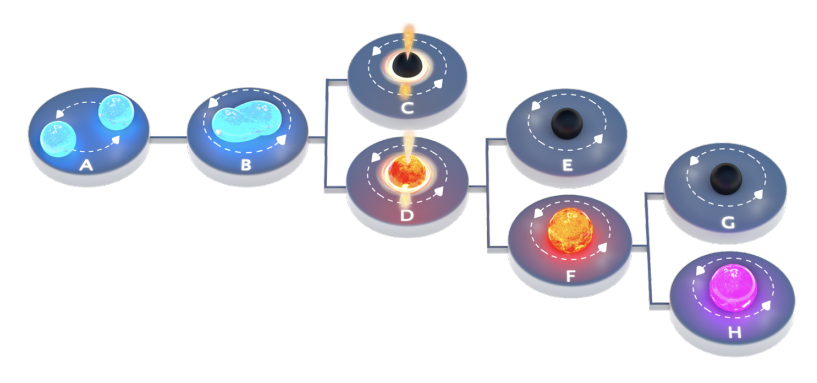
\includegraphics[scale=0.50]{images/ch2/BNS-endpoints.png}
  \caption{\fontfamily{lmss}\selectfont The evolutionary tracks of a binary neutron star mergers are thought to be dependent on the mass and rotational energy of the merger remnant. A BNS merger will either undergo prompt collapse into a black hole (A-B-C), and depending on its mass form either a meta-stable hypermassive or supramassive neutron star before collapsing into a black hole (A-B-D-E or A-B-D-F-G), or form a long-lived neutron star (A-B-D-F-H). Figure from Sarin and Lasky (2020).}
  \label{fig:BNS-endpoints}
\end{figure}

\begin{figure}[hb!]
  \centering
%   \def\svgscale{0.5}
  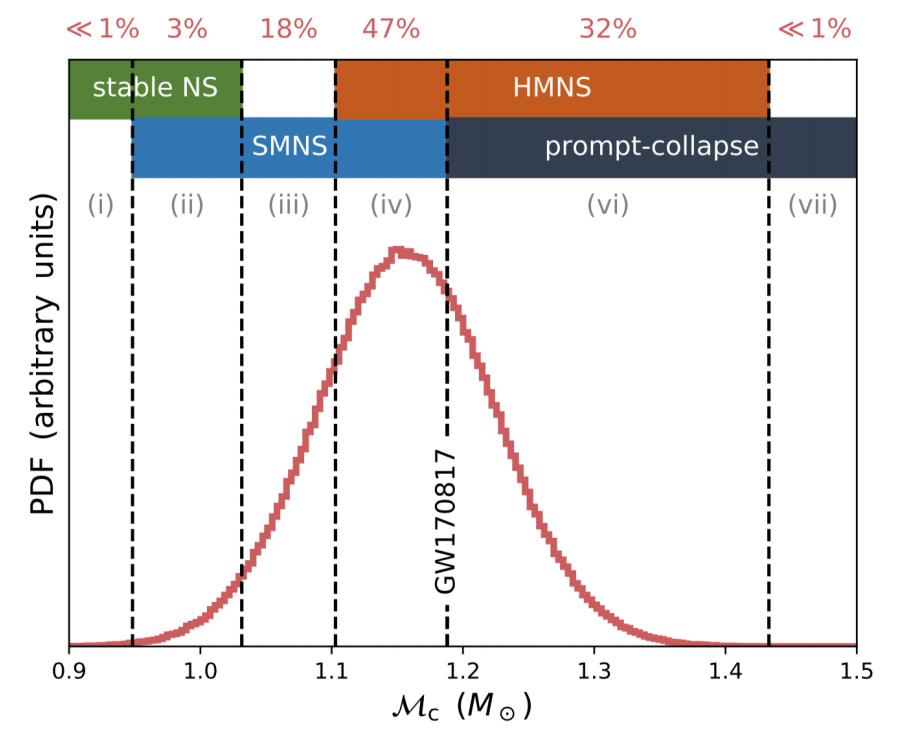
\includegraphics[scale=0.40]{images/ch2/GW170817-endpoint-PDF.png}
  \caption{\fontfamily{lmss}\selectfont A probability distribution from Metzger (2019) shows that GW170817 may have likely produced a semi-stable neutron star before collapsing into a black hole.}
  \label{fig:GW170817-endpoint}
\end{figure}
\pagebreak

\clearpage
%-------------------------2.2 All about GRBs---------------------------

\section{A Primer On Gamma-Ray Bursts}
\label{ch:Astro theory sec:GRBs}

\begin{figure}[h!]
  \centering
%   \def\svgscale{0.5}
  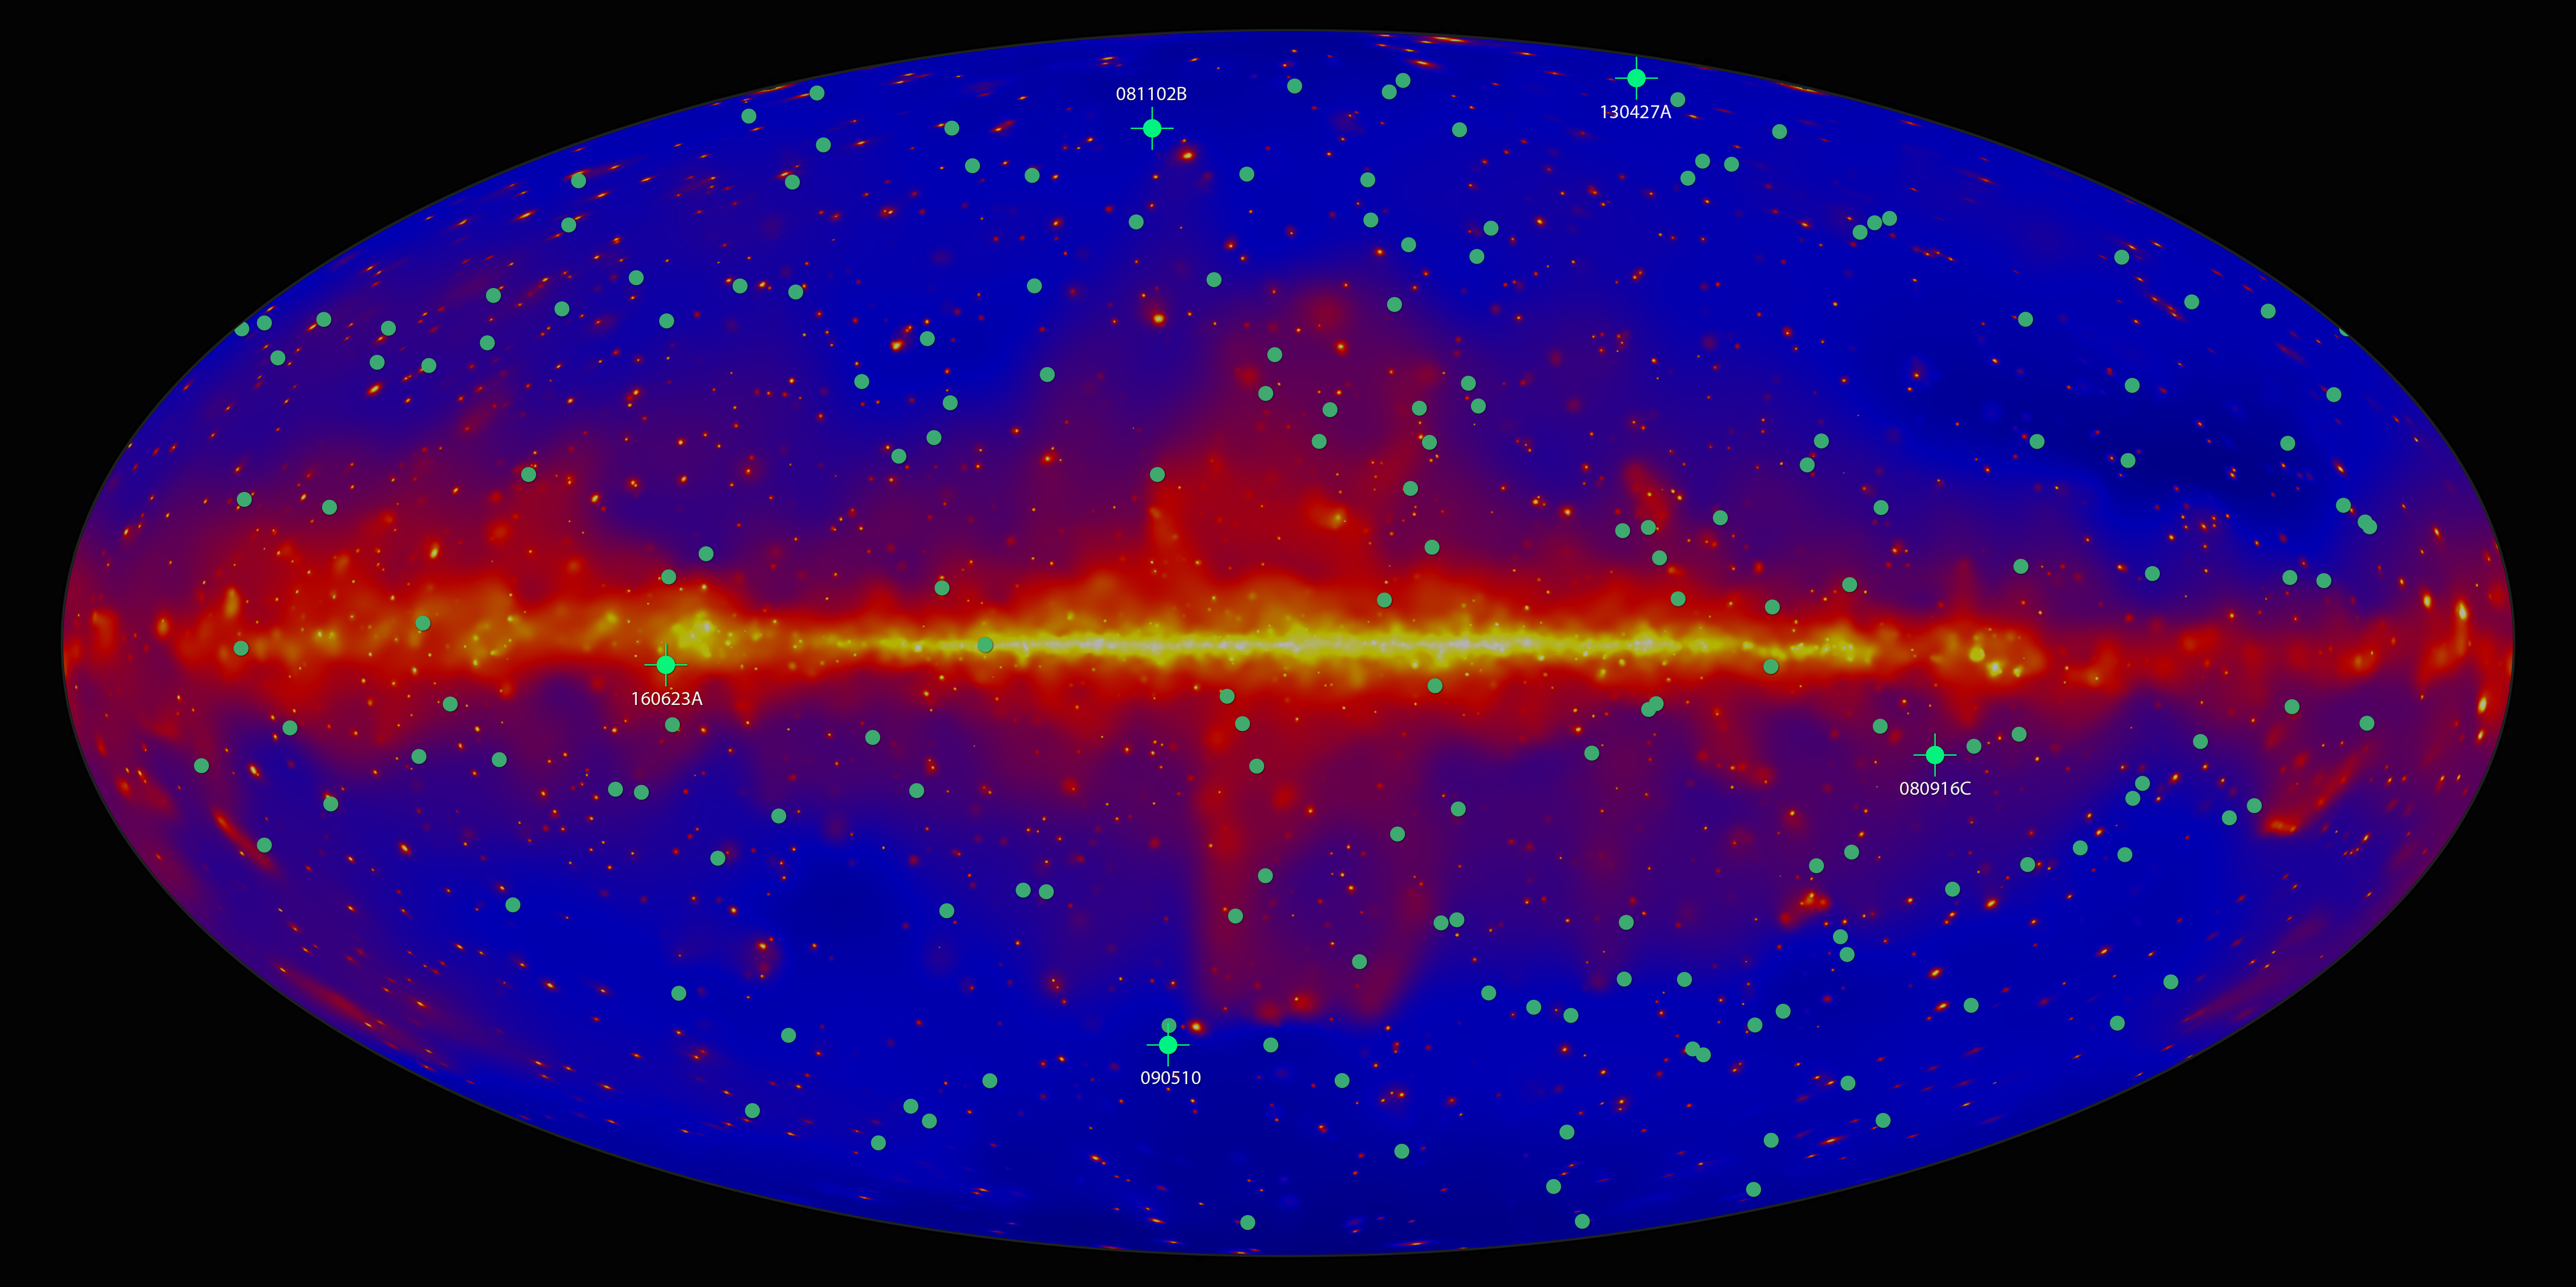
\includegraphics[scale=0.20]{images/ch2/Fermi_LAT_GRBs.jpg}
  \caption{\fontfamily{lmss}\selectfont A plot of the gamma-ray sky (observations of energies exceeding 10 GeV constructed over a period of 9 years), with the location of 186 gamma-ray bursts detected by NASA's Fermi-LAT space telescope shown in green dots. The plane of our galaxy is shown as the band in the middle of the plot. Image Credit: NASA/DOE/Fermi LAT Collaboration}
  \label{fig:GRBs Fermi-LAT}
\end{figure}

Astrophysical jets are a central phenomena in many areas of astrophysics research. They are formed in a number of different astrophysical systems, including but not limited to: pulsars, exploding stars, white dwarfs, active galactic nuclei (AGN; e.g., Bonning et al. 2012), and---as in the case of GW170817---the collision of two compact objects. Figure \ref{fig:jets} shows examples of astrophysical jets that have been observed. Gamma-ray bursts are the result of compact objects (i.e., objects on small length scales), that undergo a catastrophic event over the course of a few seconds (i.e., on small time scales), distinguishing them from other, less powerful forms of jets such as the one formed by the runaway pulsars shown in Fig. \ref{fig:jets}b and c. Gamma-ray bursts announce the birth of a highly magnetized neutron star (a magnetar) and/or a black hole via: i) the core collapse of a meta-stable hyper-massive star, ii) the merging of a binary neutron star system, or iii) the merging of a neutron star-black hole system (Venters et al. 2019). Our observations of these events are characterized as bright, non-repeating bursts of radiation spotted about once per day in random spots in the gamma-ray sky (Fig. \ref{fig:GRBs Fermi-LAT}).   


\begin{figure}[h!]
  \centering
%   \def\svgscale{0.5}
  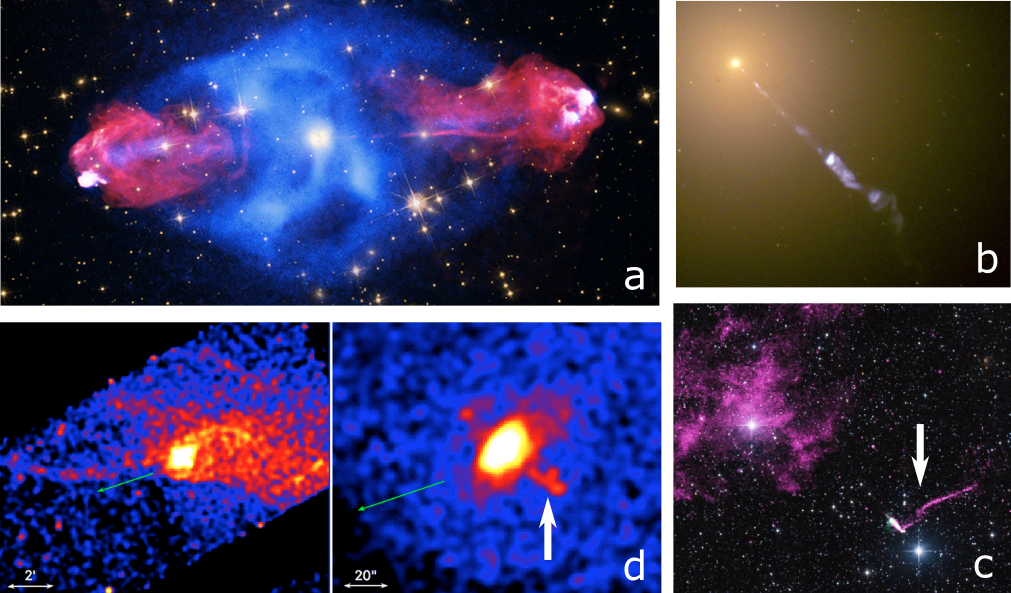
\includegraphics[scale=0.50]{images/ch2/jets.png}
  \caption{\fontfamily{lmss}\selectfont Examples of astrophysical jets in our universe: \textbf{(a)} The supermassive black hole at the cetner of Cygnus A powers twin jets, the radio emission (red) of which spans nearly 300,000 light-years across. Image Credit: NASA/CXC/SAO (X-ray), NASA/STScI (Optical), NSF/NRAO/AUI/VLA (Radio); \textbf{(b)} Messier 87 (M87) is an elliptical galaxy whose central black-hole also powers a relativistic jet. Image credit: NASA/STScI/AURA; \textbf{(c)} IGR J11014-6103 is a runaway pulsar with a trailing jet (shown in purple) 37 light-years in length. Image credit: NASA/CXC/ISDC/L.Pavan et al. (X-ray), CSIRO/ATNF/ATCA (Radio), 2MASS/UMass/IPAC-Caltech/NASA/NSF (Optical); \textbf{(d)} PSR J2021+3651 is also a runaway pulsar with smaller jets. Image credit: NASA.}
  \label{fig:jets}
\end{figure}

\subsection{A brief history}
\label{ch:Astro theory ssec:GRB hx}

Tracing the history of gamma-ray bursts takes us to the height of the race between the United States and the Soviet Union to command space and establish global hegemony, a race that began in 1957 with the Soviet launch of the first artificial satellite, Sputnik 1, into orbit. The development and successful deployment of rocket technology brought with it both the promise of space travel, and of nuclear war. To prevent the latter\footnote{\fontfamily{lmss}\selectfont The former was deferred once the Apollo program served its political ends. NASA's budget began to fall exponentially between the mid-1960s and mid-1970s.}, the Partial Test Ban Treaty was signed in 1963, and that same year the US military deployed Vela---a group of surveillance space satellites, outfitted with X-ray, gamma-ray\footnote{\fontfamily{lmss}\selectfont Gamma radiation, first discovered in the 1900s, was known to be a product one of three nuclear reactions: fusion, fission, and decay ($\alpha$- and $\gamma$-decay).}, and neutron detectors---in a highly elliptical orbit above the Earth to search for signatures of non-compliance. 

Vela first detected gamma-rays in 1967, but the data was kept classified until 1973, when Vela scientists were able to share their findings with the wider community. They had determined that the gamma-rays were cosmic in origin (i.e., not from the Earth or the Moon; Klebesadel et al. 1973), but the question of whether the signals were coming from inside our Galaxy (a galactic origin), or whether they were coming from cosmological distances was as yet unanswered. In order to settle the debate, enough GRBs needed to be observed to determine whether their distribution was concentrated in the disk of our galaxy, where the majority of stars are located, or whether they would form an isotropic distribution (i.e., observed in every direction, equally). This large-scale sampling was possible with the 1991 launch of NASA's Compton Gamma Ray Observatory (CGRO).  Only 193 days after the instrument on board, the Burst and Transient Source Experiment (BATSE), began making detections, 153 GRB events were recorded---a rate of nearly one per day. The distribution of these bursts was published in a letter in Nature and appeared to be isotropic (Meegan et al. 1992). This analysis was the beginning of the end of the debate: evidence showed that gamma-ray bursts were coming from outside of the Milky Way. A distribution of gamma-ray burst taken by NASA's Fermi-LAT is shown in Figure \ref{fig:GRBs Fermi-LAT}.

\subsection{Gamma-ray burst classification}
\label{ch:Astro theory ssec:GRB class}

Gamma-ray bursts have a wide variety of durations, time profiles, spectra, and intensities (Fishman and Meegan 1995). While no two GRBs are alike, they are known to have a bimodal duration distribution, with each class being linked to a set of unique spectral properties (Kouveliotou et al. 1993). Long GRB (LGRB) events last longer than two seconds and tend to have softer spectra, while short GRB (SGRB) events last less than two seconds and have predominantly harder spectra i.e., a burst's duration is anticorrelated with its spectral hardness (e.g., Berger 2014, Paradijs et al. 2000, Kouveliotou et al. 1993, Norris et al. 1984). The short-long divider is the observational parameter T90, the point at which 90$\%$ of the gamma-ray prompt emission counts are collected; but the division is not a clean one, as there is some overlap with the long end of SGRBs and the short end of LGRBs (Berger 2014). 

\textit{Known progenitors of GRBs.–} The bimodal distribution of GRBs imply that there are two primary populations of progenitors. LGRBs tend to be found in low-metallicity, star-forming galaxies (e.g., Levesque et al. 2010), the progenitors of which are known to be massive low-metallicity stars (Frutcher et al. 2006) that end their lives in Type Ic core-collapse supernovae (SNe Ic; Sobacchi et al. 2017, Kelly et al. 2008, see Chrimes et al. 2019 for a binary population synthesis model prescription). In other words, LGRBs are associated with recent star formation. By contrast, while around 50$\%$ of SGRBs have been observed to occur in star-forming galaxies, about 20$\%$ have been found in early-type elliptical galaxies with little to no star formation (Berger 2014, Fong et al. 2013). Looking at the ages of the stellar populations in the host galaxies of SGRBs, the timescale between the formation of the SGRB progenitor and the SGRB event is on the order of 1 Gyr (De Pasquale, 2019). Taken together, and supported by the discovery of GW170817, this is consistent with the idea that progenitors of SGRBs are two merging compact objects, either NS-NS or NS-black hole (BH)\footnote{\fontfamily{lmss}\selectfont There has not been a definitive discovery of a neutron star-black hole merger, but there was a highly probable candidate detected in 2019 (Wei and Feng 2019).}.


\subsection{Phenomenology}
\label{ch:Astro theory ssec:GRB phenom}

Our broad theoretical understanding of gamma-ray bursts requires several components, namely: a site and an environment in which to propagate, a central engine, and energy (Fishman and Meegan 1995). From decades of observation and modeling, we now know that the sites of GRBs are core-collapse supernovae and merging binary compact objects, and we can measure the environments of their host galaxies. We know that the origin of the prompt emission of GRBs is a relativistic jet and---while the central engine is something we can't observe directly\footnote{\fontfamily{lmss}\selectfont Two possible central engines are so-called black hole accretion-powered events where powered by magnetic fields, or (in the case of a BNS merger) result from a highly magnetized meta-stable neutron star (see e.g., Petropoulou et al. 2020 and references therein).}---we can infer that the amount of energy supplied to these explosions must be such that, given their cosmological distances, GRBs briefly outshine the brightest sources in our Universe. The theoretical challenge is ultimately to understand how light and relativistic matter push and pull on one another in the presence of magnetic fields, and the practical challenge is balancing the physics of relativity, radiative processes, and magnetohydrodynamics with computational resources\footnote{\fontfamily{lmss}\selectfont The most complex numerical problems are often run on supercomputers, which have a large carbon footprint. A study in Australia found that between supercomputing, flights, observatories, and office usage, astronomers have a carbon emission rate that is five times that of the national average---with more senior astronomers being the largest contributors (Stevens et al. 2020).}.  

\textit{Fireball model of GRBs.–} Gamma-ray bursts are themselves a multistage phenomenon that involve an energy source, energy transport, and energy conversion on a short timescale to the prompt emission and on a longer timescale into the afterglow (Piran 1999). Our simple model begins with a large amount of energy $E$ being injected by a central engine into a small volume with radius $r_{inj}$ (e.g., Goodman 1986, Paczy\'{n}ski 1986) that contains some amount of entrapped baryonic matter with a rest mass $M_0$. This results in an explosion with energy $E \sim \gamma_0 M_0 c^2$ and an energy-to-mass ratio of $\eta = E/M_0c^2$. Within this small volume, gamma-rays collide, increasing the temperature to a point where electron-positron pairs ($\gamma \rightarrow e^+e^-$) are formed. The pairs subsequently annihilate to produce high-energy gamma-rays  ($e^+e^- \rightarrow \gamma\gamma$). This creates an opaque energy-plasma ``soup'' called a \textit{fireball}\footnote{\fontfamily{lmss}\selectfont In our case, this is a relativistic baryonic fireball (Piran 1999) as opposed to a pure-radiation fireball.} with an optical depth $\tau \sim E \sigma_T / r_{inj}^2m_pc^2$ (where $\sigma_T$ is the Thomson cross-section) from which the photons can't readily escape (i.e., $\tau \gg 1$). Up to this point, the fireball is considered to be \textit{radiation-dominated}---its transition to the \textit{matter-dominated} phase begins with the expansion of the fireball. 

As the shell expands, energy is transferred into a relativistic matter flow with a bulk Lorentz factor $\Gamma$ that increases linearly with the radius of the fireball (Bloom 2011). The leading edge of this shell, which contains the piled up relativistic matter, has a thickness of $R/\Gamma^2$ (Van Paradijs et al. 2000), and a radius, 

\begin{equation*}
    R = \frac{R_0 \Gamma (\eta-1)^{3/2}}{(\eta - \Gamma)^{3/2}},
\end{equation}


which can be obtained through the hydrodynamic conservation of mass, momentum, and energy (see Piran 1999). Once the energy has been transferred to the particles as kinetic energy, the flow has a terminal Lorentz factor $\Gamma_0 = \eta$. At this point, the radius of the shell is sufficiently large that the fireball ``freezes out'' ($r_{freeze} \sim \eta r_{inj}$) i.e., particle motion is purely ballistic (Paradijs et al. 2000). Meanwhile, the central engine continues to episodically deposit energy, and this variability produces fireballs traveling at different Lorentz factors. As a faster shell overtakes a slower one via collisionless\footnote{\fontfamily{lmss}\selectfont The shell's radius is also sufficiently large that there is too much space between particles for them to collide head-on. Instead, energy and momentum is transferred through long-range interactions of electric and magnetic fields. This is also the case for external shocks, as we'll see with GRB afterglows.} interactions, internal shocks are produced that disrupt the particles' ballistic trajectories and converts their kinetic energy to radiation, most likely through synchrotron emission (e.g., Bloom 2011, M\`{e}sz\'{a}ros 2002). The electrons that are accelerated within these shocks take on a powerlaw distribution of energy $p$, and are thought to be responsible for the prompt GRB emissions we observe. Along with $p$, two additional dimensionless parameters that we can use to determine syncrotron emission are: $\epsilon_B$, the fraction of the magnetic field energy and $\epsilon_e$, the fraction of the total electron energy. Numerical hydrodynamics simulations (e.g., Ryan et al 2020, Eerten et al 2018, Morsony et al. 2016, MacFayden and Woosley 1999) have shown that this outflow is collimated along the axis of rotation of the central engine.    

\textit{GRB jet: structured or top-hat?–} Since GRBs are observed at cosmological distances, the fireball model, which is a spherical assumption, is valid even when considering a collimated outflow within a solid angle $\Omega_j < 4 \pi$---so long as it is observed within this angle (in this way, an observer can only see what's inside the jet; M\`{e}sz\'{a}ros 2002). This is also true for the top-hat jet model which takes this collimated form into account, and until the discovery of GW170817 has been sufficient (Ryan et al. 2020, Ryan et al. 2015). Given that GW170817 was angled with an inclination of about fifteen to thirty degrees, we viewed the event well off-axis which resulted in GRB afterglow lightcurves that were not consistent with canonical SGRBs (Lazzati et al. 2018, Mooley et al. 2018). Having opened up the potential for future joint discoveries, many of which are likely to be similarly off-axis,  we needed to refine our models to be able to make better predictions. 

A structured jet model put forth by Lazzati et al. (2017a,b) and supported by e.g., D’Avanzo et al. (2018), Troja et al. (2018), and Kasliwal et al. (2017) can help us account for this, and the semi-analytic model used in this work, developed by Lazzati and Perna (2019), will be outlined in more detail in Chapter \ref{ch:Methods}. In this model, a top-hat jet is injected with an energy $E$, and acquires structure as the head of the jet propagates through the surrounding interstellar medium through the creation of a bow shock. This bow shock surrounds the jet with a cocoon of hot material that itself is subject to shock interactions. Whether a cocoon is present, as well as its energy ($E_c$., a fraction of the total jet energy $E_c = E - E_j$) and degree of collimation (i.e, its angle $\theta_c$) is dependent on the mass of the ejecta present--the more ejecta, the more energetic and collimated and vice versa. One benefit of this model is that, in addition to accounting for off-axis viewing angle effects, it reduces to the typical top-hat structure when the viewing angle is on-axis. The utilization of structured jet models is important for our understanding of GW170817, the analysis of archival SGRBs, as well as for future observations (Ryan et al. 2020).   

\subsection{Gamma-ray burst afterglows}
\label{ch:Astro theory ssec:GRB AG}

\begin{figure}[ht!]
  \centering
%   \def\svgscale{0.5}
  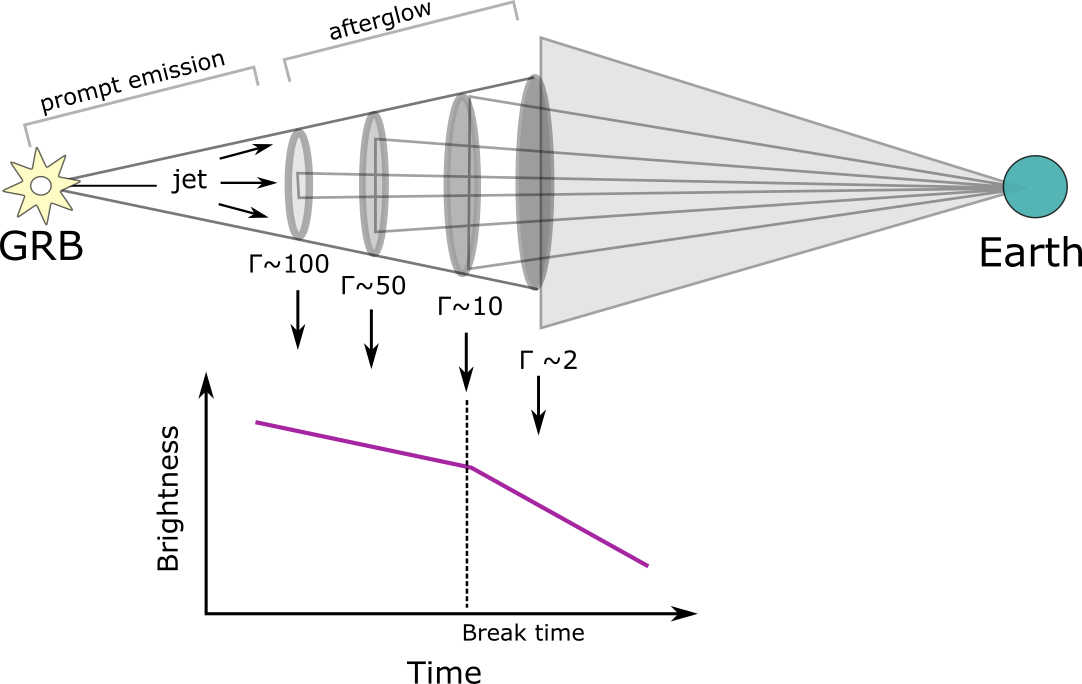
\includegraphics[scale=0.40]{images/ch2/jet-break-2.png}
  \caption{\fontfamily{lmss}\selectfont Visualization of a GRB afterglow lightcurve viewed on-axis, adapted from MacFayden (YEAR). Between $\Gamma \sim 100$ and $\Gamma \sim 50$ we see relativistic events due to the fact that we observe only a portion of the jet (the difference between the circle and triangle base). At around $\Gamma \sim 10$, we see the full width of the jet, which corresponds to a jet break. After this point, our perceived brightness decreases sharply because we now see an area that includes and extends past the jet (grey triangle). }
  \label{fig:jet-break}
\end{figure}.

A gamma-ray burst afterglow is the result of shock systems propagated by the expansion of a GRB into its environment, and are bright X-ray and radio sources in addition to being visible in optical wavelengths (van Paradijs et al 2000). As a direct result of these interactions, the afterglows we observe contain encoded information about their circumburst environments (e.g., Lazzati et al. 2019, Venters et al. 2019, Sari et al. 1998). In 1997, the study of gamma-ray bursts was revolutionized by two main events: 1) the discovery of the first GRB afterglow counterpart detected in optical and X-ray (e.g., Piro et al. 1995) following the detection of GRB970228, and 2) the first red-shift measurement made via spectroscopy of GRB970508 (e.g., Bloom et al. 2001, Metzger et al 1997)---the results of which offered further support for the cosmological distances of GRBs. Gamma-ray burst afterglows have been important for our understanding of the nature of their progenitors, they have enabled us to pinpoint a GRB's location and environment by enabling follow-up observations, and they have helped constrain the energy and geometry of the ejecta and outflow (e.g., Schady 2017). Afterglows also encode information about the intrinsic jet properties, that is properties the relativistic jet had before interacting with its surroundings (e.g., Lazzati et al. 2020, Fong et al. 2015), as well as the observer angle (e.g, Eerten and MacFayden 2012). In the case of BNS mergers, the afterglow can even be used to better understand neutron stars themselves through their equations of state (e.g., Lazzati et al. 2020, Kathirgamaraju 2019, Baiotti and Rezzolla, 2017). 

\textit{Blastwave model for GRB afterglows.–} We return again to our fireball model as it coasts with a terminal Lorentz factor $\Gamma_0$. By this time, the shell has amassed material from the surrounding environment with a particle number density $n$, such that the energy contained by that material is a significant fraction of the shell's total energy. When swept up mass contains around half of the initial explosion energy $m \sim M_0/ \gamma_0$ (van Paradijs 2000), the blast wave will begin to decelerate. The dynamics following the build-up of this external shock are described by the Blandford-McKee solution (1976), which provides a transition between pre- and post-shock conditions. The dominant form of radiation is, as in the internal shock case, due to synchrotron radiation (which produces radio, optical, and X-rays, as opposed to gamma-rays in the prompt emission) with a powerlaw distribution like the one shown in Figure \ref{fig:sync-radiation}. Note that there are complications to this simplified model, including the need to account for forward-beaming, reverse shocks, jet and limb-brightening effects (e.g., Fig. \ref{fig:jet-break}), and cases in which the circumburst medium is inhomogeneous (e.g., a disk wind outflow). How the spectrum and lightcurves resulting from the blastwave is laid out in Chapter \ref{ch:Methods sec:AG physics}.

% \clearpage
%-------------------------2.3 A corollary: GWs---------------------------

\section{A Corollary: Gravitational Waves}
\label{ch:Astro theory sec:GWs}

Hidden in the field equations\footnote{\fontfamily{lmss}\selectfont These are the equations that describe the geometry of spacetime curvature. In its most compact form, it can be expressed as $G_{\mu \nu} = -8 \pi T_{\mu \nu}$ (using the convention in which the speed of light $c$ is set equal to one). Of course, physicists are notorious for finding ways to collapse complexity--in this case, embedded in the tensor terms on the left hand side is a whole lot of it!} of Albert Einstein's theory of general relativity are the equations that describe the existence of gravitational waves (Collier 2016, Einstein and Rosen 1937).  Gravitational wave interferometry, the means by which we detect them, was a feat more than 50 years in the making---one that overcame many scientific, engineering, and political hurdles (Levin 2016) to become the LIGO scientific collaboration. Its first detection in 2015 was also our first ever detection of black holes, a vindication for Einstein a century later, as well as for the scientists who championed the completion of the LIGO project. Today the LIGO-Virgo-KAGRA collaboration, comprising thousands of researchers, technicians, and staff, is poised to begin their first joint advanced run in 2022, and will eventually be joined by a gravitational wave facility in India (e.g., Souradeep 2016).  

\textit{Gravitational wave sources.–} So far, LIGO-Virgo has only detected one type of gravitational wave---those that come from the inspiral of compact binary objects (BH-BH and NS-NS), but in theory any massive body that accelerates produces gravitational waves. Other types of GWs and their theorized sources include: stochastic gravitational waves which are thought to contain residual signals from the Big Bang, continuous gravitational waves, which would emanate from rapidly spinning massive objects like pulsars, and gravitational waves resulting from the inspiral of supermassive black holes (SMBH). 

To detect gravitational waves from SMBH binaries, which have a period of weeks to months as opposed to milliseconds as is the case for stellar-mass BHs, we turn again to our cosmic gift---the neutron star. The preciseness of radio emissions from pulsars makes them the perfect probe for detecting these kinds of GW (see e.g., Shapiro-Albert et al 2019), and the North American Nanohertz Observatory for Gravitational Waves (NANOGrav; e.g., McLaughlin 2013, Haasteren and Levin 2010) has a dedicated pulsar timing array for exactly this purpose\footnote{\fontfamily{lmss}\selectfont In a press conference early this year, NANOGrav announced that it found an intriguing signal that may be a low frequency background attributed to gravitational waves.}. NANOGrav can also be used to probe the gravitational stochastic background (Arzoumanian et al. 2018, Arzoumanian et al. 2016, Sesana et al. 2008), as well as primordial black holes (Chen et al. 2020).

\textit{A new window into astronomy and cosmology.–} Gravitational waves are being used to probe for evidence of cosmic string cosmology (e.g., Martinez and Kamai 2020), as well as for theoretical dark-matter particles called axions (e.g., Grin et al. 2020). In addition to being able to constrain the masses of the compact objects in binary systems, gravitational waves can be used to measure the eccentricities of these binary systems (e.g., Nitz et. al 2020, Lower et al. 2018, Cheeseboro and McWilliams 2015), as well as to probe the nature of the equation of state of the hot, dense matter generated in neutron star mergers (e.g., Hanauske et al. 2019, Reitze et al. 2019).

\clearpage
\section{Summary}
\label{ch:Astro theory sec:Summary}

The objective of this work is to study the nature of gamma-ray burst outflows resulting from binary neutron star mergers, which can provide insight into the intrinsic properties of the jet responsible for the prompt emission and afterglow, properties of the post-merger environment, as well as the nature of the neutron star equation of state. It is also important to be able to place the study of these phenomena in the broader context of astrophysics and cosmology. Taking these both into consideration, in this chapter we have explored the following:

\begin{itemize}
    \item The different tracks of stellar evolution, their endpoints, and how the presence of a companion star---which is the case for the majority of stars---influences their evolution.  
    \item How neutron stars are formed, how binary neutron star systems evolve, and how their collisions contain the conditions to trigger the r-process and create the heaviest elements in our Universe.
    \item Our current understanding of the physics of gamma-ray bursts, the important role observational data of their afterglows play in our understanding of BNS merger outflows. 
    \item The significance of gravitational waves beyond the detection of GW170817, and the role pulsars play in gravitational wave astronomy.
\end{itemize}



%-------------------3. Theory: The Computational Stuff--------------------------

\chapter{Markov Chain Monte Carlo Methods}
\label{ch:MCMC theory}
\begin{fquote}[Donna Haraway][1988 (p.581) ]The eyes have been used to signify a perverse capacity---honed to perfection in the history of science tied to militarism, capitalism, colonialism, and male supremacy---to distance the knowing subject from everybody and everything in the interests of unfettered power.
\end{fquote}

\textit{Overview.–} This work is grounded in a Bayesian framework, and is aided by approximations made using the numerical Markov Chain Monte Carlo (MCMC) method. These tools---made possible by the invention, advancement, and democratization of computational technologies (both hardware and software)---have transformed many fields, including those in the physical sciences, statistics, and even linguistics. Below, we will explore Bayes' theorem and MCMC in more detail and show why these tools are useful for many problems in astrophysics and cosmology. 
%-------------------3.1. STATISTICAL ANALYSIS--------------------------


\section{Probabilistic Data Analysis}
\label{ch:MCMC theory sec:PDA}



\subsection{Bayesian inference}
\label{ch:MCMC theory ssec:Baye}

\textit{Bayes' Theorem.–} At the core of Bayes' Theorem (Eq. \ref{eq:3.1}) is the idea that our beliefs can be updated with evidence. This theorem has been applied to social science experiments, is used by programmers training machine learning and artificial intelligence algorithms\footnote{\fontfamily{lmss}\selectfont We know that machine learning and artificial intelligence algorithms reproduce systems of oppression (e.g., white supremacy, abelism, heteropatriarchy; Benjamin 2019, Noble 2018, Browne 2015). One of the hidden dangers of Bayesian statistics is the inevitable application of prior knowledge, which can often be laden with subjectivity.}, as well as by scientists and engineers as a systematic tool for discerning between competing theoretical-numerical models of natural phenomena. Its central question asks: \textit{Given a set of parameters, how probable are their values given observational data?} This question can be recast in a mathematical form such that uncertainties about unknown quantities are expressed as probability distribution functions\footnote{\fontfamily{lmss}\selectfont A probability distribution function describes a bound, continuous set of possible values and likelihoods of a random number. The most well-known example of a probability distribution is the "bell curve", or normal distribution, which is centered on some mean value and spreads out in a bell shape between some minimum and maximum value (the measurement we use to quantify this ``spread", and by extension the uncertainty, is called the standard deviation).} (Lunn et al. 2012):
 \begin{equation}
P(\Theta|D)= \frac{ P(D|\Theta)P(\Theta)}{P(D)}, 
\label{eq:3.1}
\end{equation}

where $\Theta$ is a set of parameters of interest, and $D$ is our data. We can break this equation down into four components:

\begin{itemize}
\item  $ P(\Theta|D)= $  Posterior (i.e., the probability of a set of parameters given the data).  
\item $P(D|\Theta)=$  Likelihood (i.e., the probability of the data given a set of parameters).
\item $P(\Theta)=$ Prior (i.e., prior knowledge before evidence is presented).
\item $P(D)=$ Marginalization (i.e., evidence irrespective of prior knowledge).
\end{itemize}
 
With a numerical model in hand (and because we are not comparing two or more competing models), we do not need to calculate the marginalization parameter, as it will be independent of $\Theta$\footnote{\fontfamily{lmss}\selectfont Otherwise, marginalizing over all of our parameters of interest means we would be left with a multidimensional integral $P(D) = \int P(D, \Theta) d\Theta$ that would be intractable analytically, and expensive to solve computationally.} (Foreman-Mackey et al. 2013). This simplifies our equation to, 
 \begin{equation}
P(\Theta|D) \propto P(D|\Theta)P(\Theta).
\label{eq:3.2}
\end{equation}
In order to address the central question posed by Bayes' theorem, we must ask two further questions: \textit{How probable is the observed data given a set of model parameters?} and, \textit{What prior knowledge do we have of these parameters?} Oftentimes we lack prior knowledge and instead supply guesses guided by physical constraints and/or limits found in prior research, these are called \textit{uniform} or \textit{non-informative}\footnote{\fontfamily{lmss}\selectfont While it is a widely-used term, the use of ``non-informative'' is misleading because, as stated earlier, these priors are usually drawn from educated guesses.} priors. In the event priors are known, \textit{informative} priors, a distribution (e.g., a Gaussian) is provided. A mixture of informative and non-informative priors can also be used.

With the priors term taken care of, we are then left with the posterior term---which turns out to be challenging to solve analytically. We will see why this is in the next section, along with why MCMC sampling methods are invaluable for Bayesian data analysis.

\subsection{Markov Chain Monte Carlo methods}
\label{ch:MCMC theory ssec:MCMC}

\textit{History of development.–} Like the history of GRBs, the history of Monte Carlo methods, which were developed and advanced alongside the first electronic computer, has its origins in war (Metropolis, 1987). In this case, we trace the story back to the late 1940s, following the US detonation of fission bombs over Hiroshima and Nagasaki, Japan which killed hundreds of thousands of people. Scientists and engineers working at Los Alamos\footnote{\fontfamily{lmss}\selectfont There were five sites that were established for work on the Manhattan Project: Los Alamos, Met Lab, Oak Ridge, Hanford, and Columbia University. It is believed that a total of 19 Black scientists and technicians (in addition to laborers and service workers) contributed to all of the sites but Los Alamos (National Park Service, 2019). One of those people was Beatrice Parker, the first Black woman to earn a graduate degree in physics (Prescod-Weinstein 2020). They use this example as a cautionary tale for minoritized scientists, Black physicists in particular, to show that one can simultaneously break barriers and also contribute to systems of oppression.} at the time were racing to develop the fusion bomb (the hydrogen, or ``H-bomb") which would hold even deadlier capabilities than its predecessor. Computers would be instrumental in this task, as the statistical methods required for modeling complex phenomena were incredibly tedious to calculate by hand, as was done by scores of women computers.

Nicholas Metropolis and Stan Ulam (1949) were the architects behind the Monte Carlo (MC) algorithm, which they used to simulate neutron diffusion in fissionable material. Such a physical system, described by a set of differential Boltzmann equations, has a closed-form solution which is unobtainable (Metropolis and Ulam 1949, p.338), and thus could not be solved using analytical methods. They instead developed an approach that harnessed randomness to achieve a non-random (i.e., deterministic) outcome. Their statistical process, as outlined by Metropolis (1987), is illustrated here:

\begin{enumerate}
    \item Select a neutron with a random position and velocity.
    \item Independently select a position for its ``collision" with a Uranium-235 nucleus.
    \item Determine the nature of the collision:
    \begin{enumerate}
        \item If the collision results in fission, select the number of neutrons emitted and repeat the above process.
        \item If the collision results in scattering, update the neutron's momentum and repeat.
    \end{enumerate}
    \item If the neutron crosses the simulated boundary, apply boundary conditions.
\end{enumerate}

Given a sufficient amount of particles and a long enough time for the system to evolve, this approach made it possible to study the complex behavior of large systems of particles using i) simple actions as the input, and ii) without having to trace the Newtonian path of each individual particle at every time step\footnote{\fontfamily{lmss}\selectfont The computing power required to do this would be developed several years later, and molecular dynamics was introduced in 1959 (Alder and Wainwright 1959).}. 

\textit{The Metropolis method.–} The first MCMC algorithm was written by Arianna Wright Rosenbluth\footnote{\fontfamily{lmss}\selectfont Dr. Rosenbluth passed away December 28, 2020 at the age of 93.} in collaboration with Marshall Rosenbluth, Augusta Teller, and Edward Teller---all of whom knew each other through work either on the atomic or hydrogen bombs (Edward Teller would eventually become known as the ``father of the hydrogen bomb")---to improve the efficiency of the Monte Carlo method in order to simulate the equation of state of a two-phase system using a system of hard spheres. Rather than drawing independent random samples, they incorporated the ability to evolve the system in a random walk whose steps were controlled by a set of acceptance criteria. Metropolis controlled the computing resources for these simulations on the Mathematical Analyzer Numerical Integrator and Calculator, which he helped design and build. The five co-authored a paper presenting the algorithm (1953), and despite the fact that he did none of the development the algorithm came to be known as the Metropolis method, a name that obfuscated those who played the principle roles in its development.


\begin{figure}[h!]
  \centering
%   \def\svgscale{0.5}
  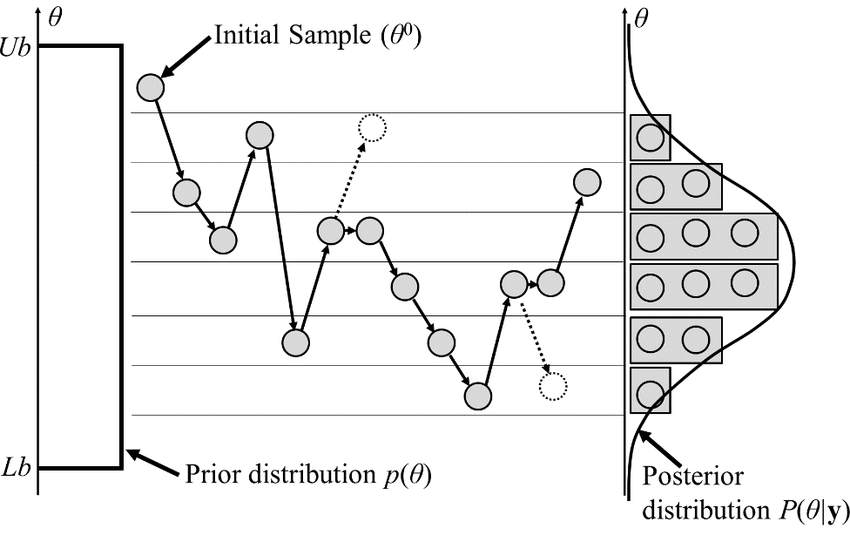
\includegraphics[scale=0.35]{images/ch3/MH-flowchart.png}
  \caption{\fontfamily{lmss}\selectfont A simplified flowchart of the Metropolis-Hastings algorithm from Lee et al. (2015). Samples are drawn from a proposal density (not shown) that fall within the upper and lower bounds ($Ub$, $Lb$) defined the prior distribution $p(\theta)$. Samples are accepted (solid grey circle) or rejected (dashed white circle), and over enough steps the samples build the posterior distribution $P(\theta|y)$. The horizontal lines show how the density of accepted samples is binned in the histogram on the right density of samples is highlighted by the horizontal lines. The initial sample is not counted in the final distribution.}
  \label{fig:MH-algo}
\end{figure}


\textit{MCMC in astrophysics and cosmology.–} MCMC methods are widely used by the astronomy community because they make it easy to sample the posterior (see: Chapter \ref{ch:MCMC theory ssec:Baye}) even in cases where the number of parameters is large i.e., a parameter space with a large number of dimensions (Foreman-Mackey et al. 2013). The most commonly used MCMC method is the Metropolis-Hastings\footnote{\fontfamily{lmss}\selectfont The ``Hastings'' component was added in 1970 (Hastings, 1970).} algorithm, with slight modifications made to improve its performance metric, the \textit{autocorrelation time}. Reducing the autocorrelation time is critical, as many problems involving the likelihood require the evaluation of numerical simulations that are resource-intensive.

To illustrate why the appeal of the Metropolis-Hastings method is so widespread, we will define the posterior and simplify our notation (following MacKay 2003) so that $P(D | \Theta) \rightarrow P(\textbf{x})$,  

\begin{equation}
    P(\textbf{x}) = \frac{P^*(\textbf{x})}{Z},
\label{eq:3.3}
\end{equation}

where $Z$ is a normalization constant,

\begin{equation}
    Z = \int d^N \textbf{x} P^*(\textbf{x}).
\label{eq:3.4}
\end{equation}

Here, $P^*(\textbf{x})$ represents the discrete form of our posterior distribution which we assume to be evaluable. We also assume that $P(\textbf{x})$ is sufficiently complex that we can't sample from it directly. This may appear to be a contradiction, however while we may be able to evaluate $P^*(\textbf{x})$, sampling $P(\textbf{x})$ is difficult for two reasons: 1) we normally don't know Eq. \ref{eq:3.4}, and 2) even with that information in hand, for problems in high dimensions we would be forced to visit every point in parameter space---a computationally expensive (and in virtually all cases, impossible) task. 

The Metropolis-Hastings method overcomes this problem by generating a random walk in a sequence of events that, given enough time to converge, will draw a representative set of samples from the posterior distribution (Fig. \ref{fig:MH-algo}; Foreman-Mackey et al. 2013). This is done through the introduction of a new, user-defined distribution, the \textit{proposal density} $Q(\textbf{x})$, whose shape is dependent on the current state in the chain. Before walking through the details of the algorithm, let's begin with a set of assumptions to help simplify the problem: 1) $Q(\textbf{x})$ is a distribution function that we \textit{can} sample from; 2) the shape of $Q(\textbf{x})$ changes as $x$ changes (i.e., $Q(\textbf{x}) \rightarrow Q(\textbf{x}' | \textbf{x})$); 3) its discrete form $Q^*(\textbf{x})$ is evaluable at any point; 4) $P^*(\textbf{x}) \propto P(\textbf{x});$ and 5) $Q^*(\textbf{x}) \propto Q(\textbf{x}).$


From here, the basic idea is straightforward: we take a random walk through the geography of the probability distribution, favoring values in parameter space with high probabilities relative to our previous state. It is this sequence of dependent events that we call a \textit{Markov Chain}. Before introducing the generalized form of the Metropolis-Hastings algorithm, we will first walk through the logic:  
\begin{enumerate}
    \item We input a starting value representing our guess. This is the first value in our Markov chain, $x^{(0)}$  
    \item We then draw two random numbers: one from a uniform distribution ranging from 0 to 1 ($u$, for later use), and one from our proposal density ($x'$, our proposed point).
    \item Before we can move from our initial guess to the proposed point, we first put that point through an acceptance test $a$. The test compares the probability of the proposed state relative to that of the current state. 
    \item If the probability of our proposed move is higher than the probability of the current state, we accept the move. The next step in the Markov chain is now $x^{(1)} = x'$, and begin the process again by drawing a new proposed point. 
    \item If, however, the probability of the proposed state was lower than that of the current state, we can still accept the move if the probability $a$ is less than the random probability $u$ we drew earlier. 
    \item If this is the case, then the move is accepted and the next step in the Markov chain is $x^{(1)} = x'$; otherwise we reject it by ``resetting" the value of the next step to that of the previous step $x^{(1)} = x^{(0)}$, and try again. 
    
\end{enumerate}

A generalized form of the Metropolis-Hastings algorithm is presented here: 

\begin{outline}
    \item Initialize $x^{(0)}$
    \item For t = 1 to T:
    \begin{outline}
        \item Sample $u \sim U{[0,1]}$
        \item Sample $x' \sim Q(x' | x) $
        \item Calculate $a = \frac{P^*(x')}{P^*(x^{(t)})}    \frac{Q(x^{(t)} | x')}{Q(x' | x^{(t)})} $
        \item If $a \geq 1$:
        \begin{outline}
            \item ACCEPT: $x^{(t+1)} = x'$
        \end{outline}
        else:
        \begin{outline}
            \item If $u < min[1, a]$:
            \begin{outline}
                ACCEPT: $x^{(t+1)} = x'$
            \end{outline}
            else: 
            \begin{outline}
                REJECT: $x^{(t+1)} = x^{(t)}$
            \end{outline}
        \end{outline}
    \end{outline}
\end{outline}

The Metropolis method is a special case of the Metropolis-Hastings method, which assumes a symmetric random walk\footnote{\fontfamily{lmss}\selectfont This reduces our acceptance test term to $a = \frac{P^*(x')}{P^*(x^{(t)})}$.}. In the case of Metropolis et al. (1953), proposals were accepted or rejected based on whether moving a particle increased or decreased the total energy of the system. Since each move in the Markov chain is dependent on the state of the previous step, the chain(s) must be run sufficiently long to generate a set of samples that can be considered to be independent samples from the posterior.

While MCMC methods have made certain classes of problems tractable, it's an iterative process that isn't necessarily efficient. Different variations of the Metropolis-Hastings algorithm vary in their difficulty of implementation as well as their rates of convergence, but the underlying goals are the same: to use them for Bayesian analysis in order to quantify uncertainties in a set of parameters given a numerical model of interest. One of these MCMC variants and it's Python implementation will be introduced in the next chapter.  

\section{Summary}
\label{ch:MCMC theory sec:Summary}

Monte Carlo methods are computational tools that rely on the generation of random numbers that are used to solve two classes of problems: 1) generating a set of samples from a probability distribution, and 2) estimating probabilistic expected values of (1). These methods have made it possible (though sometimes not entirely practical) to solve problems involving Bayesian inference. In this chapter, we have explored the following:

\begin{itemize}
    \item Bayes' theorem enables us to use statistics to improve our knowledge of a physical system, given prior knowledge (even if that knowledge is no knowledge!) and new data.
    \item Solving the posterior in Bayes' theorem can be intractable for problems with a large number of dimensions.
    \item Markov Chain Monte Carlo algorithms can be used as a way to sample a posterior distribution in a Bayesian analysis. 
    \item The sample we obtain is a discrete approximation to the posterior distribution.
\end{itemize}

%-------------------4 Methodology--------------------------


\chapter{Methodology} 
\label{ch:Methods}
\begin{fquote}[Chanda Prescod-Weinstein][2020 (p.430)]White empiricism has an impact not just on the empirical choices on the part of non-Black physicists but also on the choices of Black women physicists, including whether they continue to participate in physics at all.
\end{fquote}

\textit{Overview.–} We begin this chapter with a more in-depth look at the GRB afterglow physics introduced in Chapter \ref{ch:Astro theory ssec:GRB AG}. We then present the numerical models and Python package used for parameter estimation, the results of which are described in Chapter \ref{ch:Results}.
%-------------------4.1. AG physics equations--------------------------

\section{Afterglow emission}
\label{ch:Methods sec:AG physics}

The peak of the afterglow begins with the deceleration of the relativistic fireball through external shocks in a medium (i.e., the interstellar medium). In the comoving frame of the shock, the energy density is, 

\begin{equation}
    U' = 4\gamma^2n m_\mathrm{p}c^2,
    \label{eq:4.1}
\end{equation}

where $m_p$ is the proton mass, $n$ is the particle density, and the prime indicates the co-moving frame. The comoving magnetic field is related to the energy density by,

\begin{equation}
    B' = \sqrt{8\pi\epsilon_B U'},
    \label{eq:4.2}
\end{equation}

recall that $\epsilon_B$ is the fraction of energy density in the magnetic field. The shocks occur on a timescale, 

\begin{equation}
    t_{dec} \sim \frac{r_{dec}}{c \gamma^2} s, 
    \label{eq:4.3}
\end{equation}

where $\eta \sim E/M_0c^2$ and $r_{dec}$ is the deceleration radius,
 
\begin{equation}
    r_{dec} \sim 10^{17} E^{1/3}n^{-1/3}\eta^{-2/3} \mathrm{cm},
    \label{eq:4.4}
\end{equation}

which defines the point at which the mass of the matter swept up is equal to the rest mass of the original material (Chiang and Dermer 1999). After this point, the shell is no longer considered to be freely expanding, and the bulk Lorentz factor will first begin to decrease by a factor of $\sim$ 2 over $t_{dec} \sim r_{dec}/(c\gamma^2)$ (M\`{e}sz\'{a}ros 2002), then as a power law. The peak frequency measured in the observer frame is $\nu_m \propto \gamma B' \gamma_e^2$, where $\gamma_e^2$ is the electron Lorentz factor. This proportional relation implies that as the Lorentz factor decreases, the frequency of the radiation will as well, moving to longer wavelengths (from X-ray to radio). We can relate the minimum electron Lorentz factor $\gamma_{e,\mathrm{min}}$ to $\epsilon_e$ (the fraction of energy in the electrons) as follows, 

\begin{equation}
    \gamma_{e, \mathrm{min}} = \frac{2}{1+\mathrm{X}}\frac{m_\mathrm{p}(p-2)}{m_\mathrm{e} (p-1)}\epsilon_e \gamma, 
    \label{eq:4.5}
\end{equation}

where $X$ is the mass fraction of hydrogen and $m_e$ is the electron mass. With the magnetic field and electron energy in hand, it is now possible to calculate the syncrotron radiation spectrum $F(\nu)$ (e.g., Wijers and Galama 1999) shown in Figure \ref{fig:sync-radiation}.

Assuming the circumburst medium is uniform, the spectrum at late times, (a valid assumption as observational data from the afterglow is usually obtained hours to days after the GRB trigger), is broken down into four regions: i) a self-absorbed spectrum at low frequencies $F(\nu) \propto \nu^2$ until the self-absorption break $\nu_a$; ii) a low-frequency synchrotron slope $F \propto \nu^{1/3z}$ which breaks at $F_m \propto \nu_m$; iii) the slope decreases at higher frequencies with a shape dependent on the electron index $F \propto \nu^{-(p-1)/2}$ until a third break at the cooling frequency $\nu_c$ is reached; iv) at very high frequencies, the slope steepens as a power law $F \propto \nu^{p/2}$ as the electrons cool faster than the radius of the blastwave expands. For the break frequencies and the minimum electron energy, we see that they are all related to the same parameters of interest ($z$ is the redshift i.e., the distance from the Earth to the GRB source):

\begin{equation}
    \nu_a = f_a(\epsilon_e, \epsilon_B, n, E, p, z) \ \mathrm{Hz},
    \label{eq:4.6}
\end{equation}

\begin{equation}
    \nu_m = f_m(\epsilon_e, \epsilon_B, n, E, p, z)t^{-3/2} \ \mathrm{Hz},
 \label{eq:4.7}
\end{equation}

\begin{equation}
    \nu_c = f_c(\epsilon_e, \epsilon_B, n, E, p, z)t^{-1/2} \ \mathrm{Hz},
 \label{eq:4.8}
\end{equation}

\begin{equation}
    F_m = f_F(\epsilon_e, \epsilon_B, n, E, p, z) \ \mathrm{Hz}.
    \label{eq:4.9}
\end{equation}

From the shape of the spectra and breaks, it is now possible to compute the expected lightcurves (i.e., the time evolution of the flux) for any fixed wavelength. Below $\nu_m$, we expect that the flux increases as $t^{1/2}$ for all frequencies (van Paradijs et al. 2000). Above $\nu_m$ the flux is dependent on $p$, which early observations constrained to $p \sim 2.2-2.5$ (M\`{e}sz\'{a}ros 2002). Some of the first fits of GRB afterglows e.g. GRB970508 and GRB971214 by Wijers and Galama (1999) resulted in some of the first constraints of the environment parameters and the total energy: $\epsilon_e \sim 0.01-0.5$, $\epsilon_B \sim 0.01$, $n \sim 0.001-0.01 \ \mathrm{cm}^{-3}$, and $E_{\mathrm{TOTAL}} \sim 10^{52-54} \ \mathrm{ergs}$.    

\textit{This work.–}The numerical code used to generate afterglow lightcurves for GW170817, as well as a full list of parameters of interest (which includes and expands on the list above) will be described in Section \ref{ch:Methods ssec:AG code}.  

\begin{figure}[ht!]
  \centering
%   \def\svgscale{0.5}
  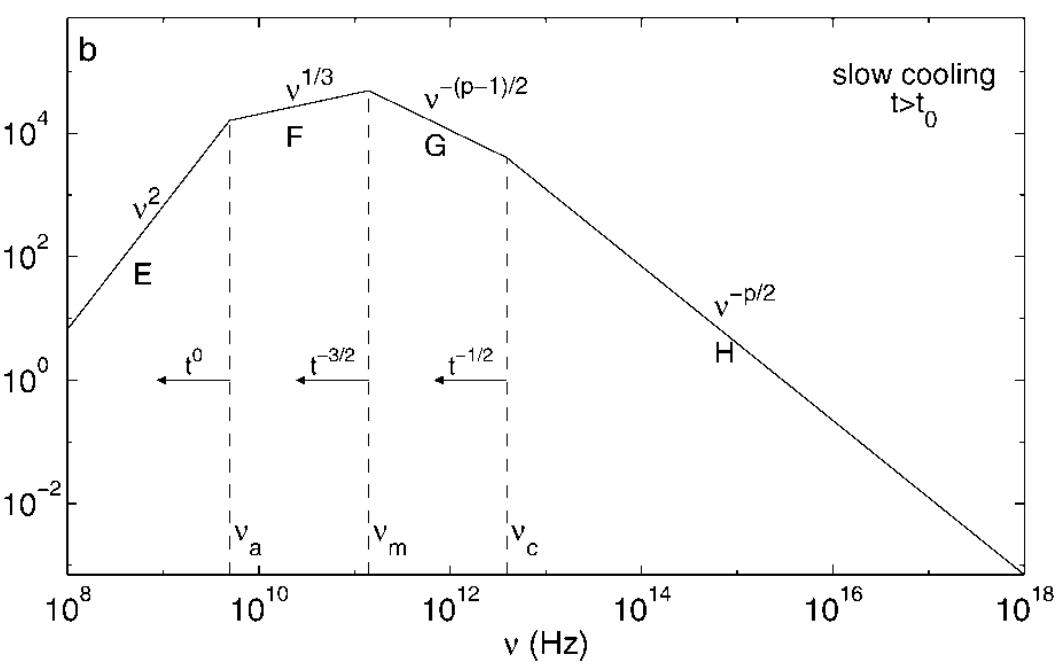
\includegraphics[scale=0.30]{images/ch4/blastwave-syncrotron-spectra.png}
  \caption{\fontfamily{lmss}\selectfont A piecewise x-ray to radio evolution from Sari et al. (1998) of the synchrotron spectrum at late times for a theoretical GRB afterglow. Note the four regions correspond to the breaks in Eq.(\ref{eq:4.6})-(\ref{eq:4.9}).}
  \label{fig:sync-radiation}
\end{figure}

%-------------------4.1. Computational Models--------------------------

\section{Computational Models} 
\label{ch:Methods sec:computational models}

\subsection{Afterglow code}
\label{ch:Methods ssec:AG code}

We used a semi-analytic model used by Lazzati et al. (2017a,b, 2018) and Perna et al. (2019) to simulate the afterglow of the SGRB associated with GW170817. The afterglow is modeled as a blastwave that expands into the surrounding interstellar medium, which is assumed to be uniform. Some major features of this model are its ability to simultaneously produce lightcurves over a set of input frequencies, the ability to define an arbitrary observer angle (i.e., a user is not limited to on-axis calculations), and the ability to supply either an analytic jet or one from a simulation; we leveraged these features to generate off-axis lightcurves in multiple radio and optical bands, as well as x-ray from a fixed distance of 40 Mpc.  

\textit{Structured jet profiles.–} The afterglow code described above incorporates profiles of the Lorentz factor $\Gamma$ and isotropic energy $E_{iso}$ associated with a jet-cocoon structure. We used the profiles prescribed by Lazzati and Perna (2019). The profile of the isotropic energy is a double-exponential given as,

\begin{equation}
    \frac{E_{iso}}{4 \pi} = \frac{dE}{d\Omega} = Ae^{-\frac{\theta}{\theta_j}} + Be^{-\frac{\theta}{\theta_c}},
   \label{eq:4.10}
\end{equation}

where $\theta_j$ and $\theta_c$ are the opening angles of the jet and cocoon respectively and are free parameters in the afterglow model. The constants $A$ and $B$ are determined by the energy of each component, 

\begin{equation}
    E_j = A \int_\Omega e^{-\frac{\theta}{\theta_j}} d\Omega,
    \label{eq:4.11}
\end{equation}

\begin{equation}
     E_c = B \int_\Omega e^{-\frac{\theta}{\theta_c}} d\Omega.
     \label{eq:4.12}
\end{equation}

The profile for the Lorentz factor is given as, 

\begin{equation}
    \Gamma = \Gamma_0 e^{ -\frac{\theta}{\theta_j}} + \Gamma_c e^{ -\frac{\theta}{\theta_c}} + 1,
   \label{eq:4.12}
\end{equation}

where $\Gamma_0$ is a free parameter of the model, and $\Gamma_c = \Gamma_0/10$. 

\begin{figure}[ht!]
  \centering
%   \def\svgscale{0.5}
  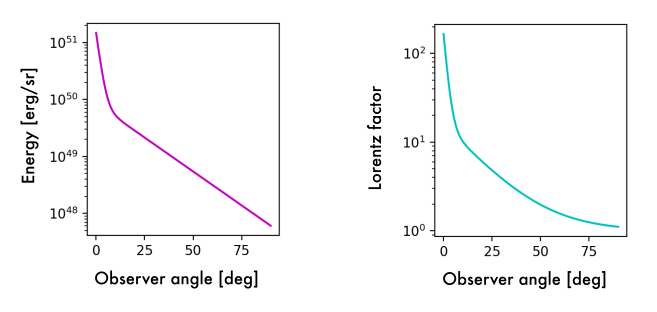
\includegraphics[scale=0.80]{images/ch4/profiles.png}
  \caption{\fontfamily{lmss}\selectfont Example of Lorentz and energy profiles used to outfit the afterglow code with a structured jet.}
  \label{fig:sync-radiation}
\end{figure}

\textit{Multiband observational data.–} The dataset used to determine the wavelengths used by the afterglow code came from the dataset compiled by Makhathini et al. (2021). Refer to Chapter \ref{ch:Conclusion sec:source code} for where to find this dataset. Due to the sparse nature of the observations, a cleaning script was developed to create a masked array of data that would be compatible with {\fontfamily{qcr}\selectfont emcee} (see Eq. \ref{eq:4.15}). One of the limitations of this afterglow code is that the addition of a wavelength to calculate also increases the time it takes the code to compute the lightcurves, so an effort was made to use as many wavelengths as possible while remaining mindful of model runtime. In total, we used 7 wavelengths: 5 in radio, 1 in optical, and 1 in X-ray (Table \ref{table:multiband dataset}).

\textit{Input.–} A detailed list of free parameters used in this code can be found in Table \ref{table:AG params}. The free parameters were selected to probe information about: the circumburst environment ($n_{ISM}$), the structured jet ($E_j$, $E_c$, $\theta_j$, $\theta_c$, $\Gamma_0$), jet microphysics ($\epsilon_e$, $\epsilon_B$, $p_{index}$) as well as the observer angle $\theta_{obs}$ For completeness, the {\fontfamily{qcr}\selectfont emcee} parameters used for this code are shown in Table \ref{table:emcee-AG params}. We fixed both the distance to GW170817 (40 Mpc), as well as the seven wavelengths to calculate that were picked from our dataset.

\textit{Output: Lightcurves.–} Our outputs of interest were the flux density (in Jy) and time (in s) for each of the wavelengths of interest, as required by Eq. \ref{eq:4.15}. Figure \ref{fig:sample-lightcurves} shows an example of the lightcurves generated by the afterglow code, compared to datapoints used from the Mooley dataset. 

 \begin{figure}[ht!]
\begin{center}
	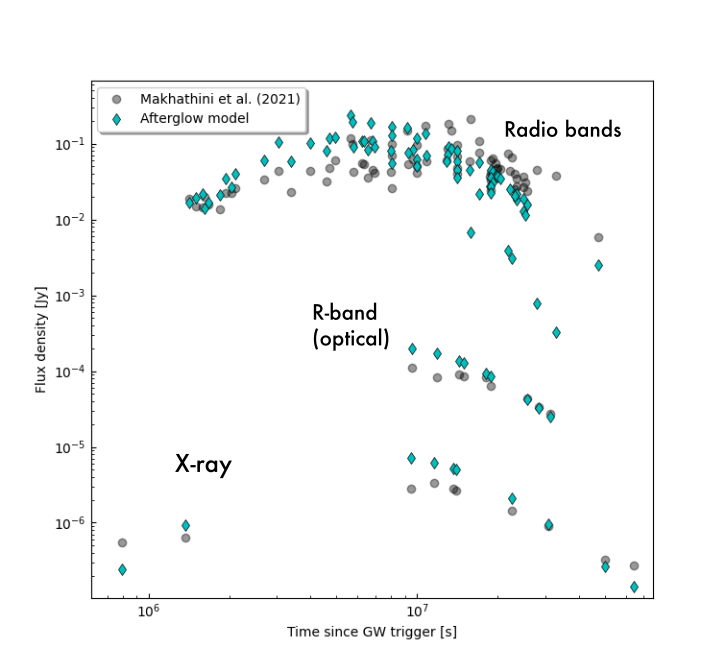
\includegraphics[width=10cm]{images/ch4/DL_lightcurves.png}
	\caption{\fontfamily{lmss}\selectfont Sample lightcurves calculated by our afterglow model (blue diamonds) compared to the observational dataset (radio, optical, X-ray; black circles).}
	\label{fig:sample-lightcurves}
	\end{center}
\end{figure}

%  \begin{figure}[ht!]
% \begin{center}
% 	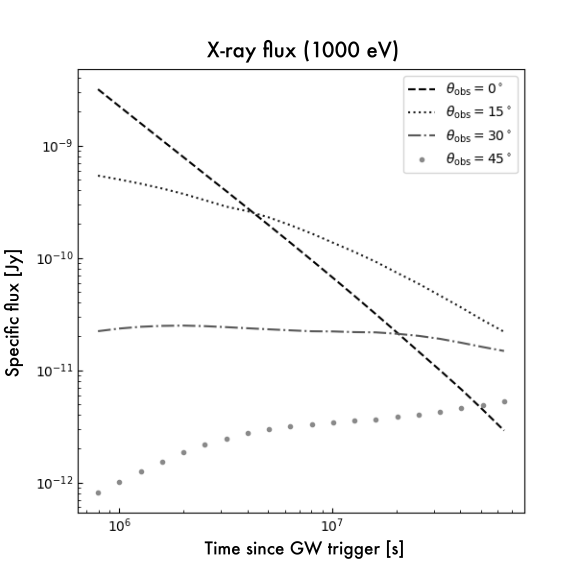
\includegraphics[width=10cm]{images/ch4/x_ray_flux.png}
% 	\caption{\fontfamily{lmss}\selectfont Flux in the X-ray band plotted generated by our afterglow model for a range of observer angles.}
% 	\label{fig:x-ray-flux}
% 	\end{center}
% \end{figure}

\subsection{Outflow code}
\label{ch:Methods ssec:outflow code}

Because of the role dynamical ejecta plays in the formation of a relativistic outflow, we employ a parameter estimation analysis of the semi-analytic outflow model developed by Lazzati and Perna (2019). The model follows the idea that a meta-stable neutron star was created, but does not distinguish between whether the jet was launched by a black hole or a HMNS (Lazzati et al. 2020). This is because in either case the NS ejecta, modeled as non-relativistic wind, is ejected into the surrounding environment before the relativistic jet is launched. Parameters of interest include those from the NS ejecta ($\dot m_w$, $v_w$), central engine ($\Delta_t$, $T_{engine}$), and jet at injection ($\theta_0$, $\Gamma_0$, $L_0$).

\textit{Input.–} A detailed list of free parameters used in this code can be found in Table \ref{table:outflow params}. For completeness, the {\fontfamily{qcr}\selectfont emcee} parameters used for this code is shown in Table \ref{table:outflow-emcee params}

\textit{Data.–} A subset of results from our afterglow-{\fontfamily{qcr}\selectfont emcee} fits for the following variables were used for the outflow-{\fontfamily{qcr}\selectfont emcee} run: $E_j$, $E_c$, $\theta_c$, and $\Gamma_0$. The $50^{th}$ percentiles of the samples in the marginalized distributions were used as data, while the $16^{th}$ and $84^{th}$ percentiles were used to calculate uncertainties.

\textit{Output.–} As required by Eq. \ref{eq:4.15}, the jet-outflow model outputs of interest are $\theta_j$, $\theta_c$, and $E_c$ from which $E_j$ can be calculated as $E_j= (L_0 T_{engine}) - E_c$. 

%------------Afterglow tables methods--------------------------------

\begin{table}[htbp!]
\caption{\fontfamily{lmss}\selectfont Free model parameters used in the semi-analytic GRB afterglow code.}
\centering
\begin{tabular}{cccc}
\hline\hline
%  & & &  \\
\textbf{Parameter} & \textbf{Class} & \textbf{Description} & \textbf{Units} \\
\hline
$\epsilon_e$ & jet microphysics & fraction of energy of electrons &  -- \\
\hline
$\epsilon_B$ &  jet microphysics & fraction of energy of magnetic field &  -- \\
\hline
$p_{index}$ &  jet microphysics & electron slope &  -- \\
\hline
$n$ & environment & external number density of ISM & -- \\
\hline
$E_j$ & jet & relativistic (core) jet energy & ergs \\
\hline
$E_c$ & jet &  relativistic cocoon energy & ergs \\
\hline
$\theta_j$ & jet & jet opening angle & deg \\
\hline
$\theta_c$ & jet & cocoon opening angle & deg \\
\hline
$\Gamma_0$ & jet & terminal Lorentz factor & -- \\
\hline
$\theta_{obs}$ & observer & observer angle & deg \\

\hline
\hline
\end{tabular}
\label{table:AG params}
\end{table}

\begin{table}[ht]
\caption{\fontfamily{lmss}\selectfont The set of multiband observational data used in the afterglow analysis.} % title of Table
\centering  % used for centering table
\begin{tabular}{ccc} % centered columns (2 columns)
\hline\hline                        %inserts double horizontal lines
\textbf{Band} & \textbf{Frequency} & \textbf{Number of datapoints} \\  %[0.5ex] inserts table heading
\hline                  % inserts single horizontal line
3.00 GHz & Radio & 20  \\ % inserting body of the table
6.0 GHz & Radio & 11  \\
4.50 GHz & Radio & 7   \\
15.0 GHz & Radio & 4  \\
11.0 GHz & Radio & 4 \\
2.42 $\times 10^{17}$ Hz & X-ray & 10 \\
4.99 $\times 10^{14}$ Hz & Optical & 9 \\
\hline  
\end{tabular}
\label{table:multiband dataset} % is used to refer this table in the text
\end{table}

\begin{table}[ht]
\caption{\fontfamily{lmss}\selectfont Parameters used by {\fontfamily{qcr}\selectfont emcee} for the afterglow model.} % title of Table
\centering  % used for centering table
\begin{tabular}{cc} % centered columns (2 columns)
\hline\hline                        %inserts double horizontal lines
\textbf{{\fontfamily{qcr}\selectfont emcee} parameter} & \textbf{value} \\  %[0.5ex] inserts table heading
\hline                  % inserts single horizontal line
walkers & 200  \\ % inserting body of the table
iterations & 10,000  \\
dimensions & 10  \\
move & stretch (default) \\ % [1ex] adds vertical space
\hline  
\end{tabular}
\label{table:emcee-AG params} % is used to refer this table in the text
\end{table}

% \clearpage
%-----------------Outflow tables methods------------------------


\begin{table}[htbp!]
\caption{\fontfamily{lmss}\selectfont Free model parameters used in the semi-analytic outflow code.}
% \tablefootnote{ISA: refer to this website while finalizing table style: https://people.inf.ethz.ch/markusp/teaching/guides/guide-tables.pdf}
\centering
\begin{tabular}{cccc}
\hline\hline
%  & & &  \\
\textbf{Parameter} & \textbf{Class} & \textbf{Description} & \textbf{Units} \\
\hline
$\dot m_w$ & NS ejecta & mass loss & \(M_\odot\) /s \\
\hline
$v_w$ & NS ejecta & wind velocity & c \\
\hline
$\theta_0$ & jet & jet angle at injection &  deg \\
\hline
$\Gamma_0$ & jet & Lorentz factor at injection &  -- \\
\hline
$L_0$ & jet & luminosity at injection & erg/s \\
\hline
$\Delta t$ & jet engine & time delay to jet launch & s \\
\hline
$T_{engine}$ & jet engine & activity time of the central engine & s \\
\hline
\hline
\end{tabular}
\label{table:outflow params}
\end{table}

\begin{table}[ht]
\caption{\fontfamily{lmss}\selectfont Parameters used by {\fontfamily{qcr}\selectfont emcee} for the outflow model.} % title of Table
\centering  % used for centering table
\begin{tabular}{cc} % centered columns (2 columns)
\hline\hline                        %inserts double horizontal lines
\textbf{{\fontfamily{qcr}\selectfont emcee} parameter} & \textbf{value} \\  %[0.5ex] inserts table heading
\hline                  % inserts single horizontal line
walkers & 100  \\ % inserting body of the table
iterations & 10,000  \\
dimensions & 7  \\
move & stretch (default) \\ % [1ex] adds vertical space
\hline  
\end{tabular}
\label{table:outflow-emcee params} % is used to refer this table in the text
\end{table}
\clearpage


\section{Bayesian Parameter Estimation Code}
\label{ch:Methods sec:Bae PE code}

Recall from Chapter \ref{ch:MCMC theory ssec:Baye} our need to calculate the expected value of a posterior probability function defined in Eq. \ref{eq:3.2}, as well as our need for efficiency for problems with a large number of dimensions. The open-source {\fontfamily{qcr}\selectfont emcee} package was engineered for this purpose, and is a popular tool in the astrophysical literature, which includes work by Kirichenko et al. (2015) on PSR J2021+3651, a runaway pulsar with jets shown in Figure \ref{fig:jets}d. While an MCMC method could have been implemented from scratch, leveraging a well-engineered (robust and tested), open-source alternative is preferable as the availability of source code leads to citability, standardization, and most importantly, reproducibility. Below, we will walk through the algorithm behind {\fontfamily{qcr}\selectfont emcee} and how it differs from the Metropolis-Hastings algorithm.   

% work on replacing emcee with \mintinline{python}{emcee} with black lettering and white background!

\subsection{The {\fontfamily{qcr}\selectfont emcee} python package}
\label{ch:Methods ssec:about emcee}

The MCMC Hammer\footnote{\fontfamily{lmss}\selectfont A play on the rapper MC Hammer, arguably most famous for his song \href{https://www.youtube.com/watch?v=otCpCn0l4Wo}{U Can't Touch This}. This example highlights the juxtaposition of the hypervisibility and consumption of Blackness in popular culture with the historical exclusion and invisibility of Blackness in physics and astronomy---and in the sciences more generally. Incidentally, MC Hammer was a celebrity supporter of the ``Black in X Week" movement that swept Twitter following the \#ShutDownSTEM protests led by ShutDownSTEM in collaboration with Particles for Justice and VanguardSTEM. The ``Black in X Week" movement was started by \href{https://www.nasa.gov/faces-of-nasa/ashley-walker}{Ashley L. Walker} who founded \#BlackinAstro Week as a way to increase the visibility of Black scholars, including junior scholars.}: {\fontfamily{qcr}\selectfont emcee} (Foreman-Mackey et al. 2013) is a Python implementation of the ``stretch move''---an affine-invariant ensemble sampling method for Markov Chain Monte Carlo. The stretch move algorithm outperforms the Metropolis-Hastings algorithm and was first proposed by Goodman and Weare (2010).

Affine-invariance of an algorithm refers to its ability to perform well under a linear transformation, making it insensitive to any covariance present between parameters (Foreman-Mackey et al. 2013). Whereas traditional MCMC algorithms move one variable at a time through a Markov chain, the Goodman-Weare algorithm utilizes an ensemble of ``walkers" where each step in the Markov chain is an iterative cycle through all $N$ walkers. Each walker $X_k$ has its new position updated in a way that is dependent on the current position of each of the other walkers (these other walkers comprise a separate, complementary ensemble). This is because it is assumed that each of the walkers contain information about the target density (our posterior). 

Walking through the algorithm to update the position of a walker $X_k$ we,
\begin{enumerate}
    \item Draw a random walker from the complementary ensemble $X_j (j \neq k)$
    \item Draw a random variable Z from a distribution g(Z=z) with an adjustable scaling parameter $a =2$, where 
    \[
    g(z) \propto  
    \begin{cases}
        \frac{1}{\sqrt{z}},& \text{if } z \in \left[ \frac{1}{a}, a\right]\\
            0,              & \text{otherwise.}
    \end{cases}
    \]

    \item Propose a new position $X_k(t) \rightarrow Y = X_j + Z[X_k(t)-X_j]$
    \item Draw a random number from the distribution [0,1]
    \item Accept or reject the proposed move with probability (as in the Metropolis-Hastings algorithm),
    \begin{equation*}
        q = min\left(1, Z^{n-1} \frac{p(Y)}{p(X_k(t)}\right)
    \end{equation}
    \item If the random number is less than q, accept ($X_k(t+1) \rightarrow Y$). Else, reset ($X_k(t+1) \rightarrow X_k(t)$).
\end{enumerate}

\begin{figure}[ht!]
  \centering
%   \def\svgscale{0.5}
  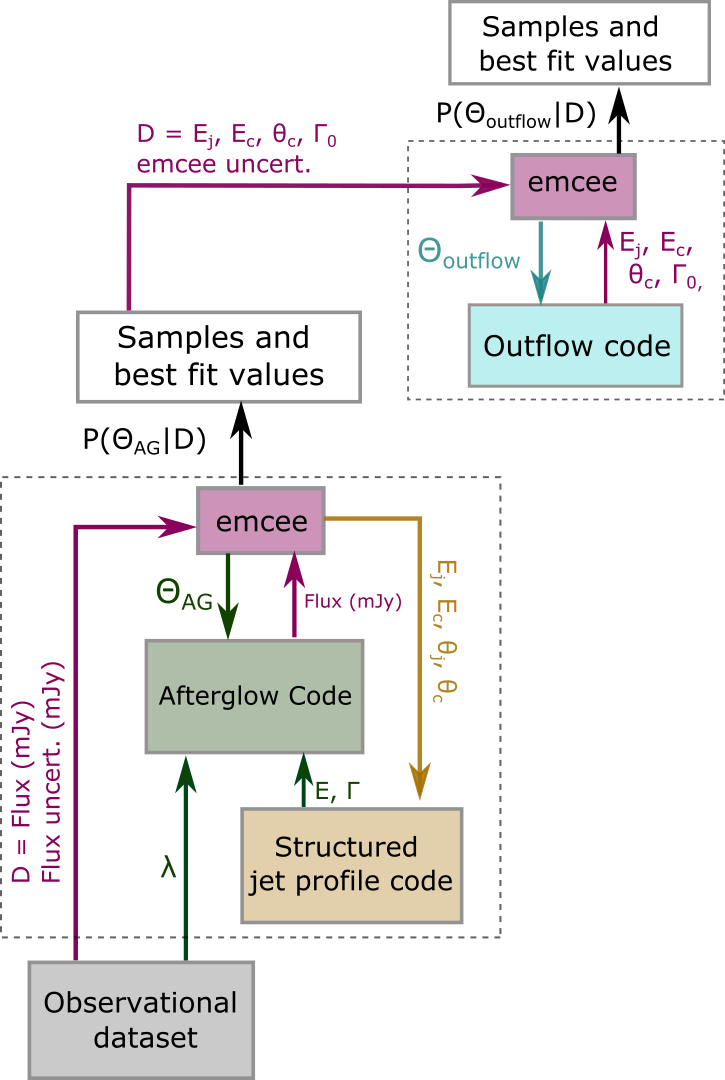
\includegraphics[scale=0.65]{images/ch4/block-diagram.png}
  \caption{\fontfamily{lmss}\selectfont A block diagram outlining the flow of how our models were used with {\fontfamily{qcr}\selectfont emcee} in order to perform Bayesian parameter estimation. $D$ represents the data used, $\Theta$ is the set of free parameters, and $P(\Theta | D)$ is our posterior.}
  \label{fig:block-diagram}
\end{figure}

\clearpage

\subsection{How it works}
\label{ch:Methods ssec:how emcee works}
Before we can run {\fontfamily{qcr}\selectfont emcee}, we first need to set up the probability function that we want to sample. Because {\fontfamily{qcr}\selectfont emcee} uses the log of the posterior, Eq. \ref{eq:3.2} becomes,

\begin{equation}
    \mathrm{ln}(p(\Theta | D) = \mathrm{ln}(p(\Theta) + \mathrm{ln}(p(D|\Theta)),
    \label{eq:4.14}
\end{equation}

where our log prior $p(\Theta)$ is, 

    \[
    \mathrm{ln}p(\Theta_i) =  
    \begin{cases}
        0,& \text{if } \Theta_{i, LB} \leq \Theta_i\leq \Theta_{i, UB}\\
            - \infty,              & \text{otherwise,}
    \end{cases}
    \]

for each parameter $\Theta_i$ in the set $\Theta$, where LB and UB stand for the lower and upper bounds of the flat prior distribution. The log likelihood is, 

\begin{equation}
    \mathrm{ln}(p(D | \Theta)) = -\frac{1}{2}\sum_i \left( \frac{\mathrm{data} - \mathrm{model \ output}}{\mathrm{data \ uncertainty}}\right).
    \label{eq:4.15}
\end{equation}

The data and its uncertainties are defined as variables (i.e., these values are static). However the numerical model will take as inputs values of the free parameters generated by {\fontfamily{qcr}\selectfont emcee} as it takes a random walk through parameter space (e.g., Fig. \ref{fig:MH-algo}). It is this step that can be the most resource intensive if the model takes even on the order of minutes to complete one iteration. Results are continuously stored in a backend hdf5 file, enabling the user to monitor progress of the Markov chains. Once the {\fontfamily{qcr}\selectfont emcee} run has completed, the samples and autocorrelation time can be pulled from this backend file and plotted using the {\fontfamily{qcr}\selectfont corner.py} (Foreman-Mackey, 2016). {\fontfamily{qcr}\selectfont emcee} documentation can be found at \href{https://emcee.readthedocs.io/en/stable/}{https://emcee.readthedocs.io}. 



\section{Summary}
\label{ch:Methods sec:Summary}

The objectives of our work are twofold: to constrain a large set of jet, observer, and environmental parameters using a rigorous numerical afterglow model, and to use the results of the jet parameters to constrain a different set of parameter estimates using a numerical outflow model. To accomplish this, we ran two separate Bayesian fits using the {\fontfamily{qcr}\selectfont emcee} MCMC sampler to obtain representative samples of the posterior distribution functions, which are presented and discussed in Chapter \ref{ch:Results}. Our generalized procedure using the {\fontfamily{qcr}\selectfont emcee} Python package is described below:

\begin{itemize}
    \item Identify an afterglow dataset of interest, and use its flux densities and measurement uncertainties for a set of wavelengths of interest.
    \item Define the generative model function that utilizes a structured jet profile and identify a set of free parameters $\Theta$ of interest for that model, keeping a fixed distance to GW170817.
    \item Define the main {\fontfamily{qcr}\selectfont emcee} functions: {\fontfamily{qcr}\selectfont logPrior}, {\fontfamily{qcr}\selectfont logProbability}, and {\fontfamily{qcr}\selectfont logLikelihood}.
    \item Initialize walkers around an initial guess for each free parameter. Run the sampler over $n$ iterations, using a backend file to monitor results. 
    \item Once a run has completed $n$ iterations, pull the samples from the backend file and plot them using the {\fontfamily{qcr}\selectfont corner.py} module.
    \item To obtain a parameter's best estimated value, use the $50^{\mathrm{th}}$ percentile of the marginalized distribution. Use the$16^{\mathrm{th}}$ and $84^{\mathrm{th}}$ percentiles as its lower and upper uncertainties. 
    
\end{itemize}

%----------------------5. RESULTS-------------------------------

\chapter{Results} 
\label{ch:Results}
\begin{fquote}[National Science Foundation][2018] Between the years 1973 and 2015, less than one hundred Black women were awarded PhD's in Physics. Less than 10 were awarded to Indigenous women.
\end{fquote}

Results from both the afterglow and jet-cocoon models are summarized in table form as well as in corner plots. The histograms in the diagonal of the corner plots show the marginalized posterior probability density functions $p(\Theta | D)$, and the inner triangle shows the posterior probabilities. The three dashed lines represent best fit values and uncertainties from the $16^{\mathrm{th}}$, $50^{\mathrm{th}}$, and $84^{\mathrm{th}}$ quantiles. These results will be discussed in Section \ref{ch:Results sec:Discussion}. 

%-----------------5.1 Afterglow--------------------------------

\section{Afterglow code}
\label{ch:Results sec:AG code}

 \begin{figure}[ht!]
\begin{center}
	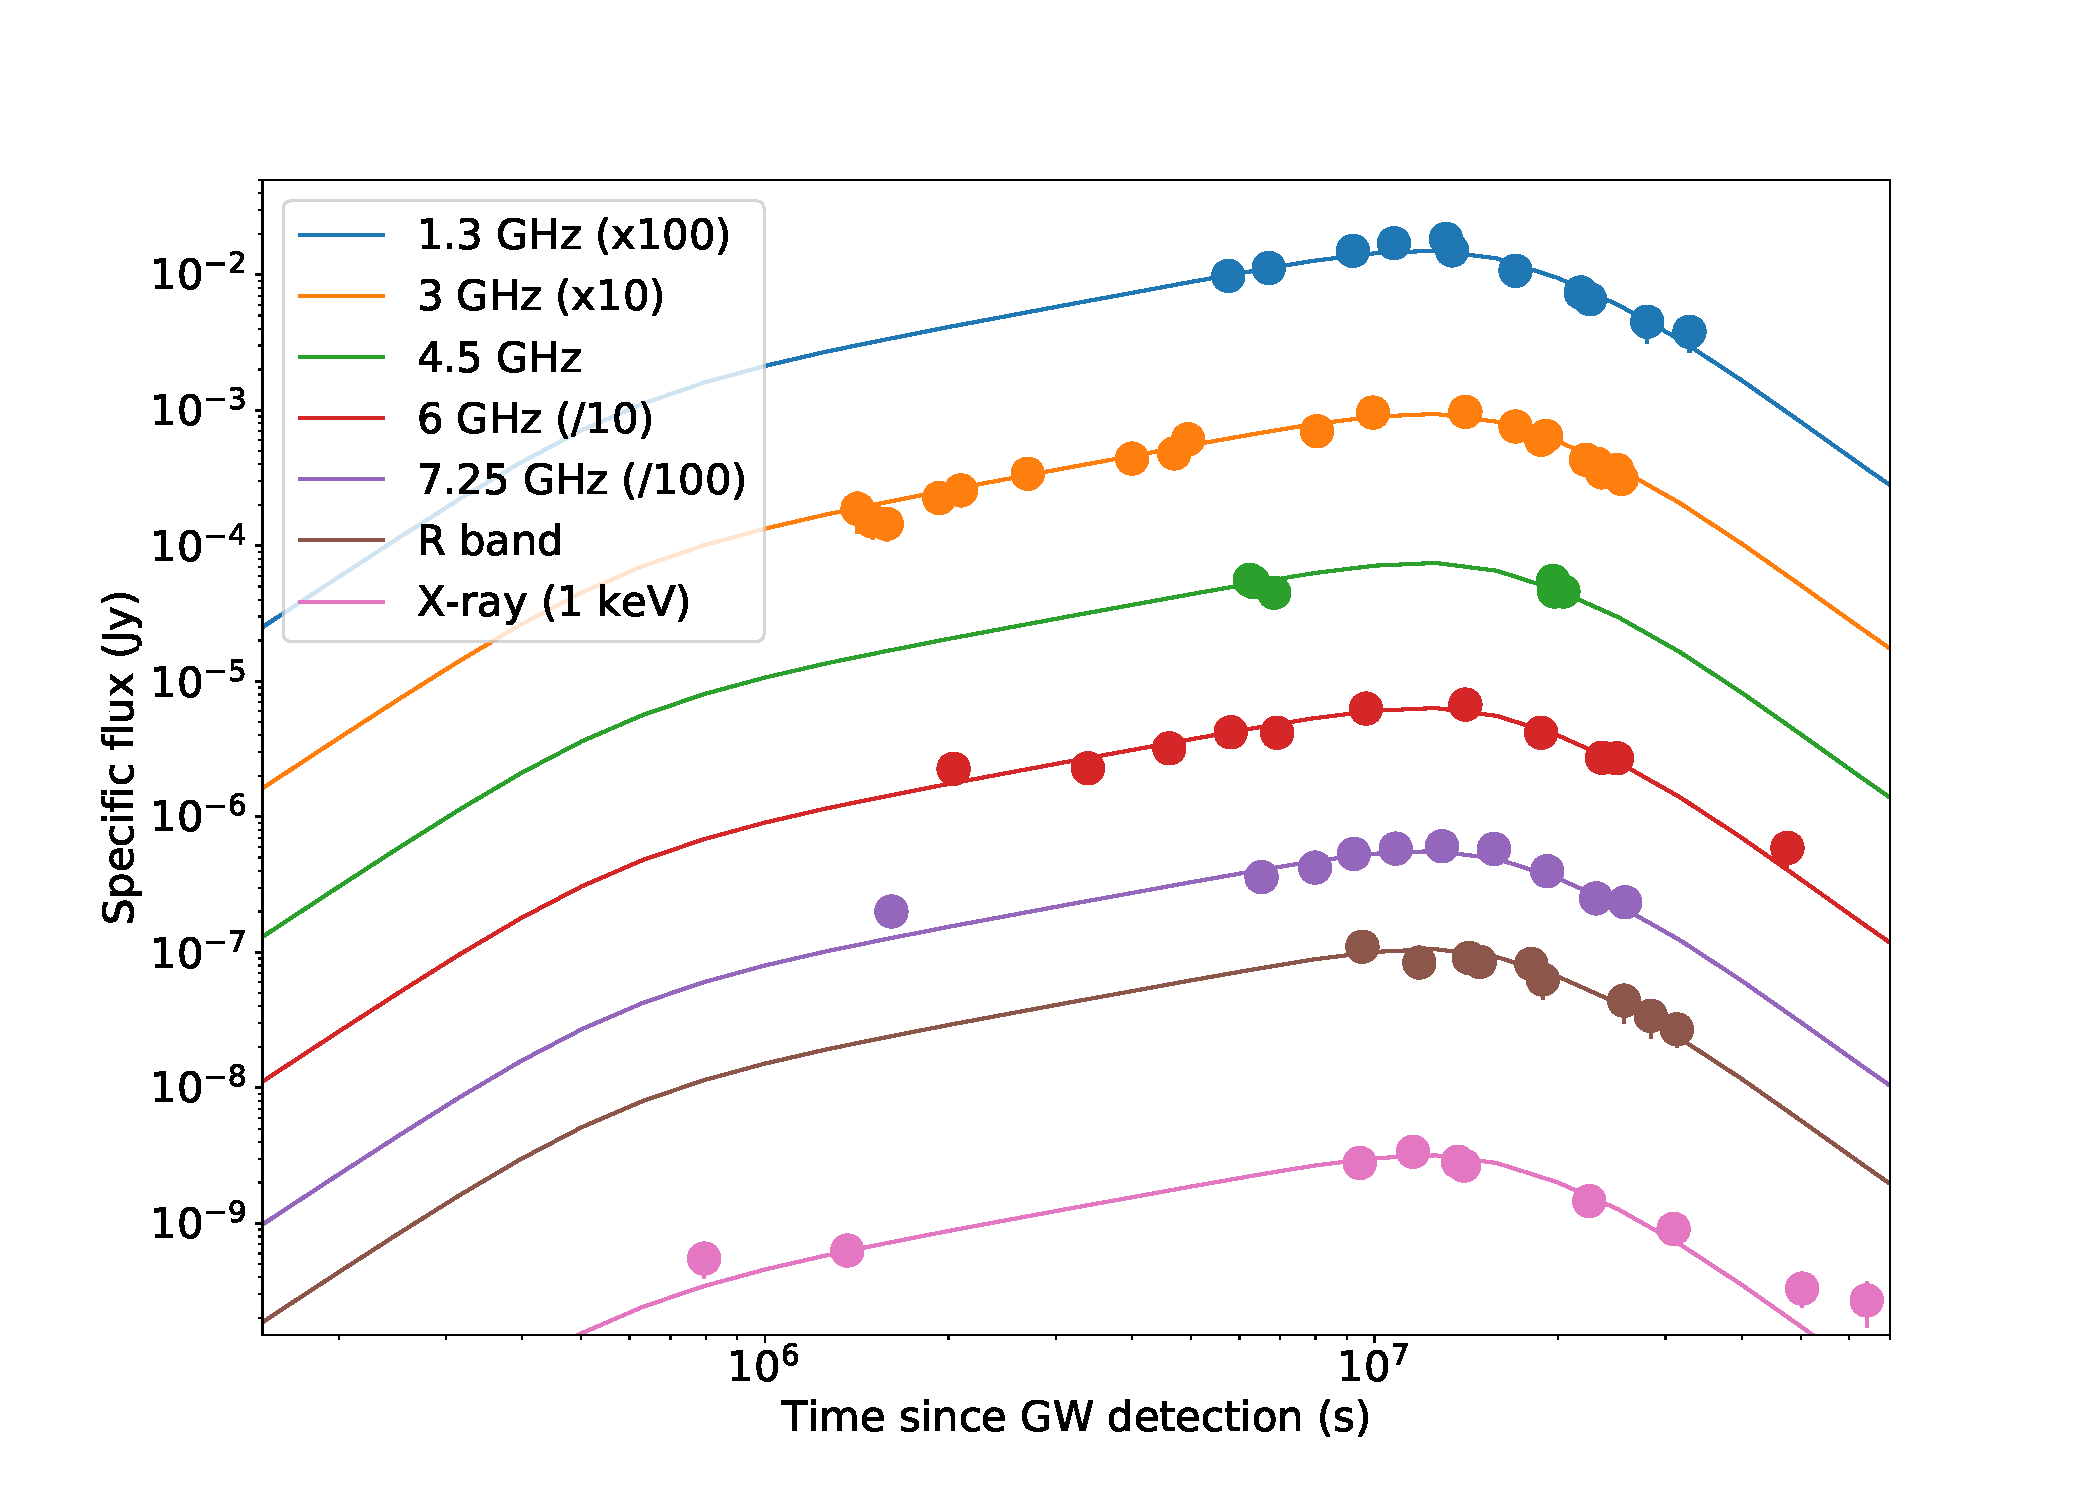
\includegraphics[width=14cm]{images/ch5/best_fit.pdf}
	\caption{\fontfamily{lmss}\selectfont Sample lightcurves generated by our afterglow model, using using the following {\fontfamily{qcr}\selectfont emcee} parameter proposals: $log(\epsilon_e) = -1.45$, $log(\epsilon_B) = -2.28$, $p_{index} = 2.13$, $log(n_{ISM} = -3.23$, $log(E_j) = 49.58$, $log(E_c) = 47.90$, $\theta_j = 1.66$, $\theta_c = 4.25$, $log(\Gamma_0) = 3.97$, $\theta_{obs} = 24.41$. This combination resulted in a log-likelihood of -38.82, indicating a good fit. The first five lightcurves are radio bands, followed by optical (R-band) and X-ray. The scattered points are observational data (converted from mJy). The colors of the observational data points correspond to same frequencies in the model data.}
	\label{fig:final-lightcurves}
	\end{center}
\end{figure}

   For our multiband study using the numerical afterglow model, we use a flat prior distribution using the parameters listed in Table \ref{table:emcee-AG params} to obtain the posterior distributions shown in Figure \ref{fig:emcee-JB}. We found that we were able to constrain the jet angle to $\theta_j = 2.51^{+0.80}_{-0.58}  \ \mathrm{degrees}$, as well as the energy of the jet $E_j \approx 6.76 \times 10^{49} \ \mathrm{ergs}$ and cocoon $E_C \sim 3.24 \times 10^{48} \mathrm{ergs}$. Our analysis established a lower limit of the terminal Lorentz factor, with a best fit value of $\Gamma_0 \sim 3500$. While the jet angle was well constrained, we found that the cocoon angle was not well constrained ($\theta_c = 14.57^{+7.24}_{-7.04}  \ \mathrm{degrees}$) in addition to showing signs of degeneracy with other model parameters (namely, $\theta_j$ and $\theta_{obs}$). The observing angle, which was constrained to $29.45^{+6.94}_{-5.96} \ \mathrm{degrees}$, is in agreement (within the errors) with the ranges found in the literature. The parameters describing the jet's microphysics, $\epsilon_e$, $\epsilon_B$, and $p_{index}$ were also well constrained and in agreement with the literature. A complete list of the best fit values resulting from our Bayesian parameter estimation of the afterglow is summarized in Table \ref{table:emcee-AG best values}. An example snapshot of model vs data fits in the {\fontfamily{qcr}\selectfont emcee} sampling chain is shown in \ref{fig:final-lightcurves}.

%-----------------5.2 Outflow--------------------------------

\section{Outflow code}
\label{ch:Results sec:Outflow code}

Similar to our afterglow study, jet-cocoon outflow model, we use a flat prior distribution using upper and lower bounds determined by the afterglow fits and the parameters listed in Table \ref{table:outflow-emcee params} to obtain the posteriors shown in Figure \ref{fig:emcee-outflow}. We found that we were able to constrain the mass loss rate to $\dot m_w \approx 0.05$ \(M_\odot\)/s, as well the jet parameters at injection: $L_{0} \approx 7 \times 10^{49} \ \mathrm{erg/s}$ and $\Gamma_{inj} \sim 1445$. Our model favored an engine duration of $T_{\mathrm{engine}} \gtrsim 1.26 \ \mathrm{s}$. We also obtained upper limits on the time delay to jet launch $\Delta_t \lesssim 0.41 \ \mathrm{s}$ and the wind velocity $v_w \lesssim 0.15c$. A list containing the final best fit values for all of the parameters are summarized in Table \ref{table:emcee-outflow best values}.  

\begin{figure}
\begin{center}
	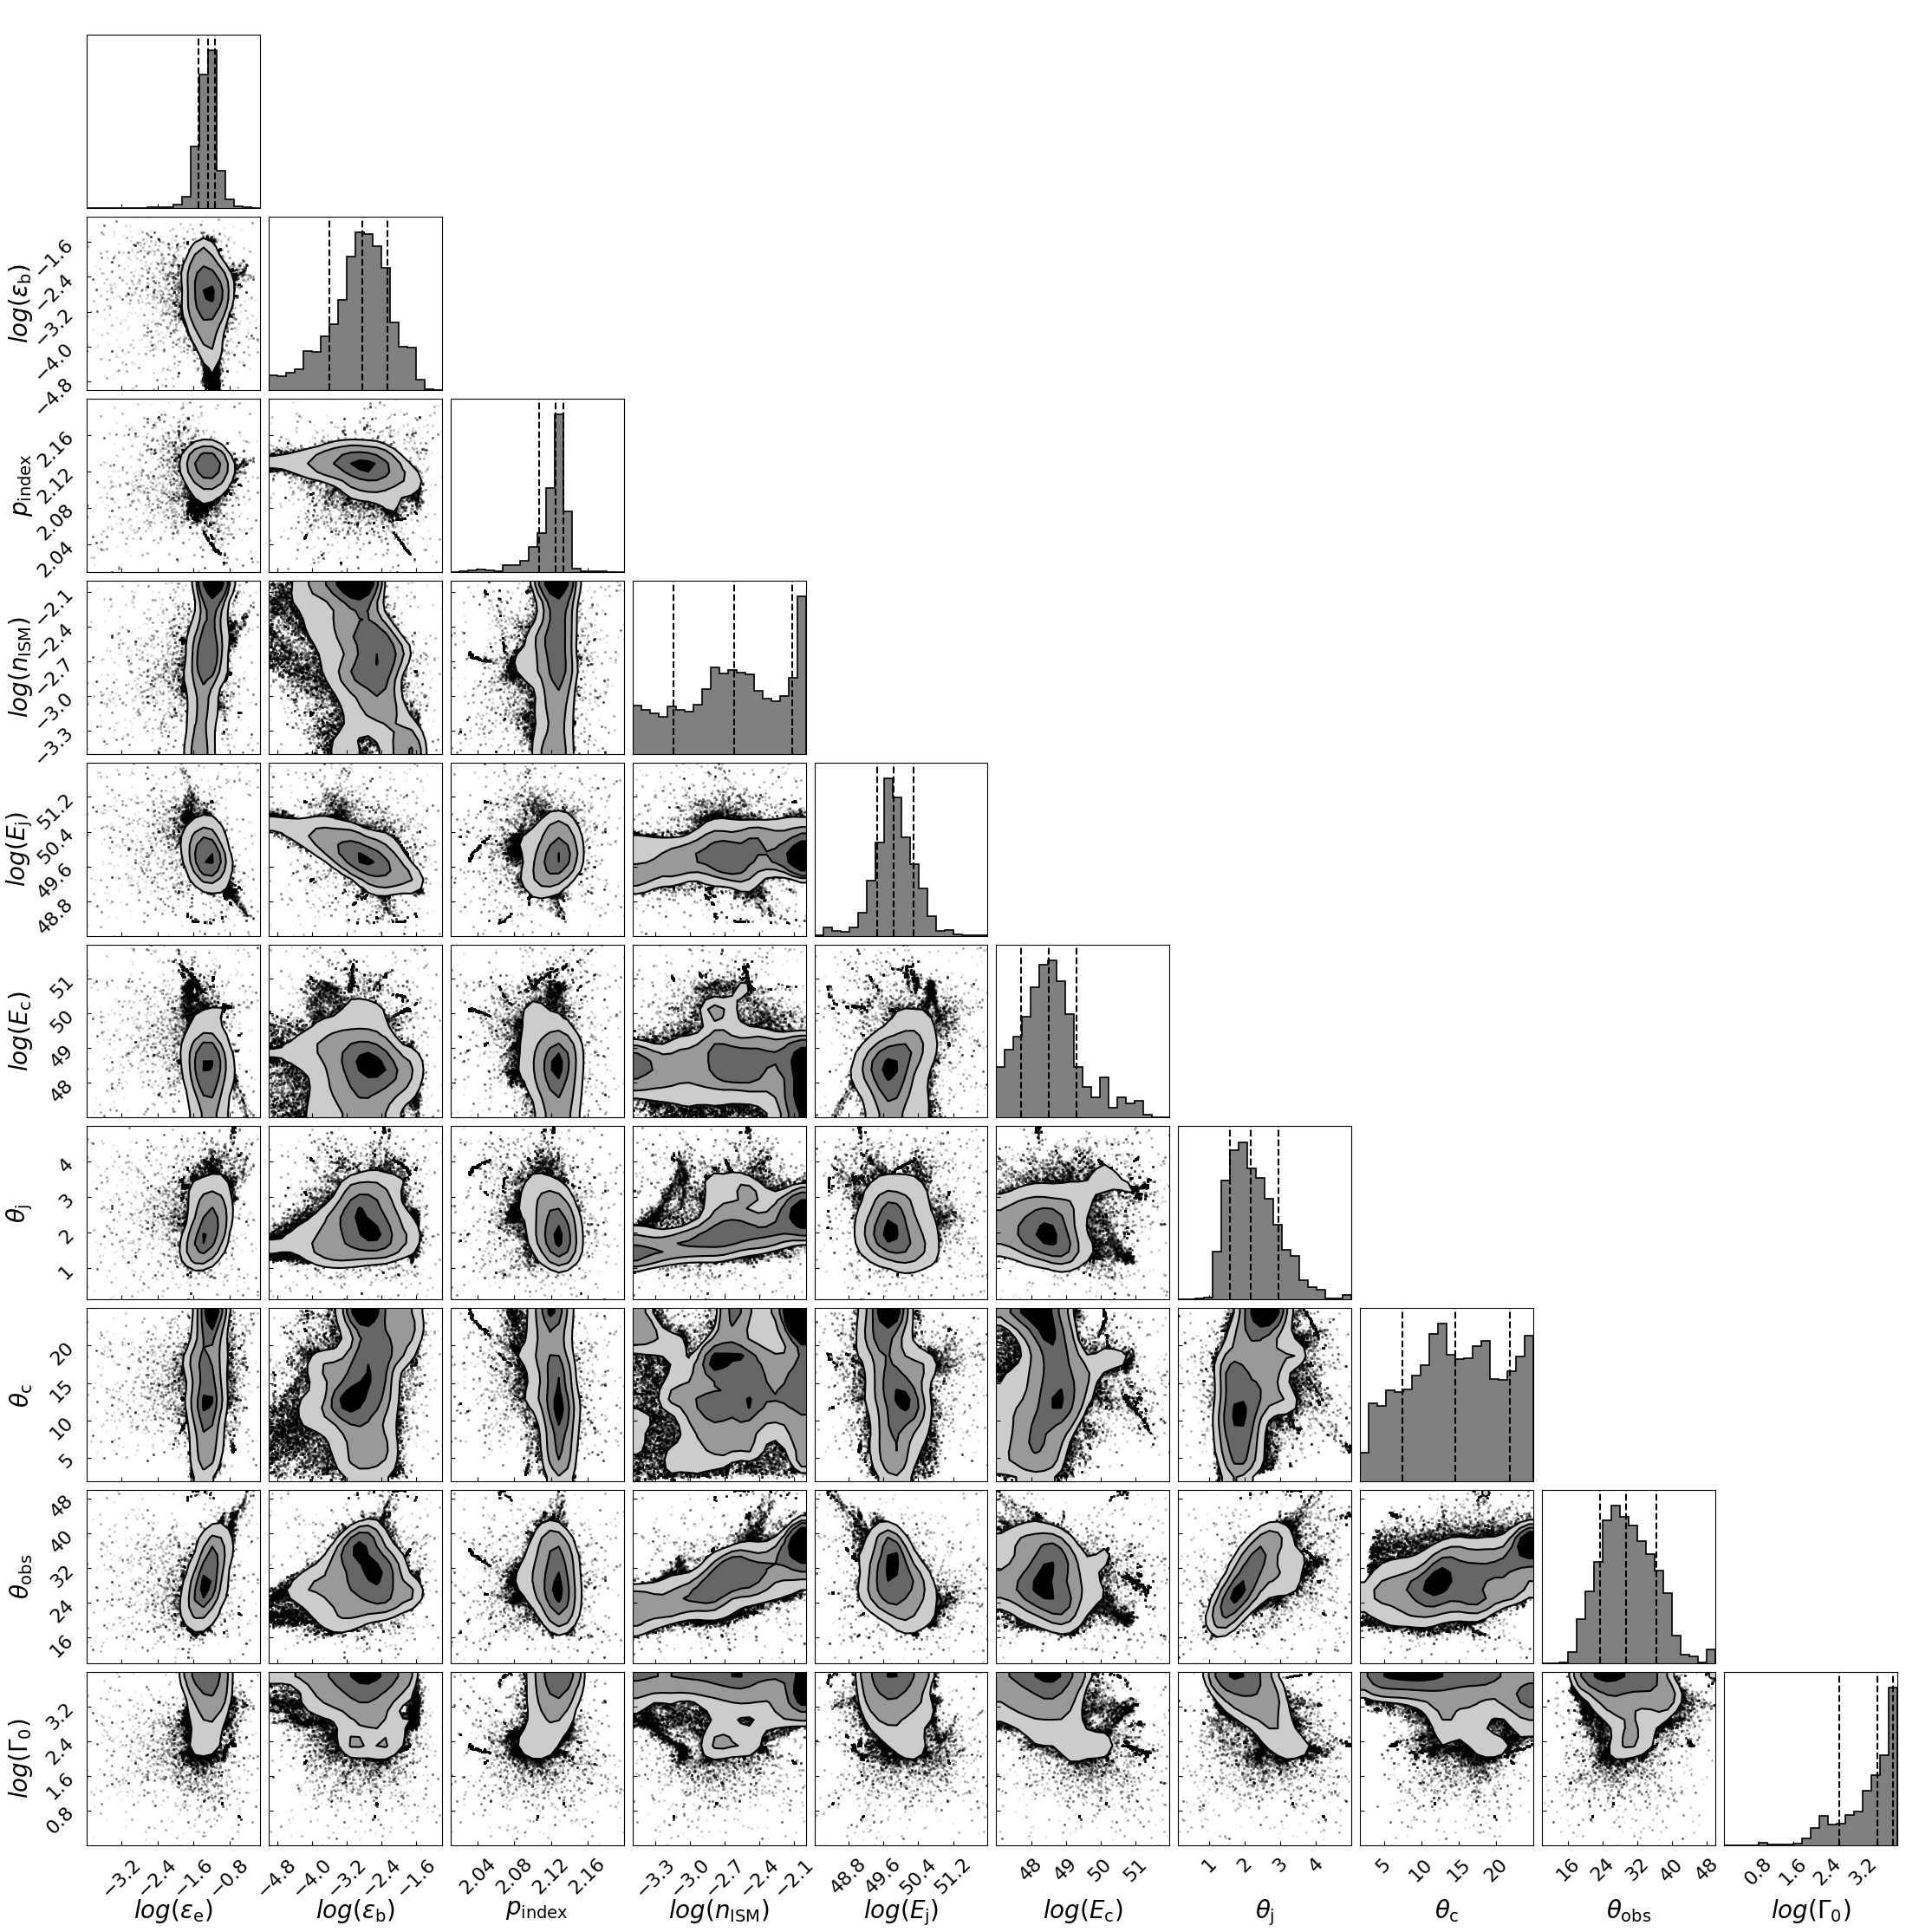
\includegraphics[width=15cm]{images/ch5/mcmc_DL.png}
	\caption{\fontfamily{lmss}\selectfont Preliminary posterior distributions obtained by applying observational data  constraints to our structured jet afterglow model. The histograms in the diagonal of the corner plots show the marginalized posteriors and the inner triangle shows the posterior probabilities. The dashed lines indicate the $16^{\mathrm{th}}$, $50^{\mathrm{th}}$, and $84^{\mathrm{th}}$ quantiles respectively.}
	\label{fig:emcee-JB}
	\end{center}
\end{figure}
\pagebreak[4]

\begin{table}[htbp!]
\caption{\fontfamily{lmss}\selectfont Bayesian parameter estimation results using our afterglow model.}
% \tablefootnote{some kind of footnote from a table, which doesn't work without the tablefootnote package}
\centering
\begin{tabular}{cccc}
\hline\hline
%  & & &  \\
\textbf{Prior bounds} & \textbf{{\fontfamily{qcr}\selectfont emcee} estimate} & \textbf{Units} & \textbf{Description} \\
\hline   \\
$ -4 \leq log(\epsilon_e) \leq -0.3$ & $-1.29^{+0.16}_{-0.21}$ & -- & fraction of energy of electrons \\
\\
\hline 
\\
$ -4 \leq log(\epsilon_B) \leq -0.3$ & $-2.84^{+0.57}_{-0.76}$ & -- & fraction of energy of magnetic field  \\
\\
\hline 
\\
$2 \leq p_{index} \leq 2.5$ & $2.13^{+0.01}_{-0.02}$ & -- & electron slope \\
\\
\hline 
\\
$-4 \leq log(n_{ISM}) \leq -0.3$ & $-2.62^{+0.50}_{-0.52}$ & $\mathrm{cm^3}$ & external number density of ISM  \\
\\
\hline 
\\
$-4\leq log(E_j) \leq 50$ & $49.83^{+0.46}_{-0.37}$ & erg & relativistic (core) jet energy \\
\\
\hline 
\\
$-4 \leq log(E_c) \leq 49$ & $48.51^{+0.80}_{-0.80}$ & erg & relativistic cocoon energy \\
\\
\hline 
\\
$0 \leq \theta_j \leq 10$ & $2.15^{+0.80}_{-0.58}$ & deg & jet (core) opening angle \\
\\
\hline 
\\
$\theta_j + 0.6 \leq \theta_c \leq 20$ & $14.57^{+7.24}_{-7.04}$ & deg & cocoon opening angle  \\
\\
\hline 
 \\
$-4\leq log(\Gamma_0) \leq 2.70$ & $3.54^{+0.36}_{-0.89}$ & -- & terminal Lorentz factor \\
 \\
\hline
\\
$0 \leq \theta_{obs} \leq 90$ & $29.45^{+6.94}_{-5.96}$ & deg & observer angle \\ [1ex]
\hline
\hline
\end{tabular}
\label{table:emcee-AG best values}
\end{table}
\pagebreak[4]

\clearpage

\begin{figure}[h!]
\begin{center}
	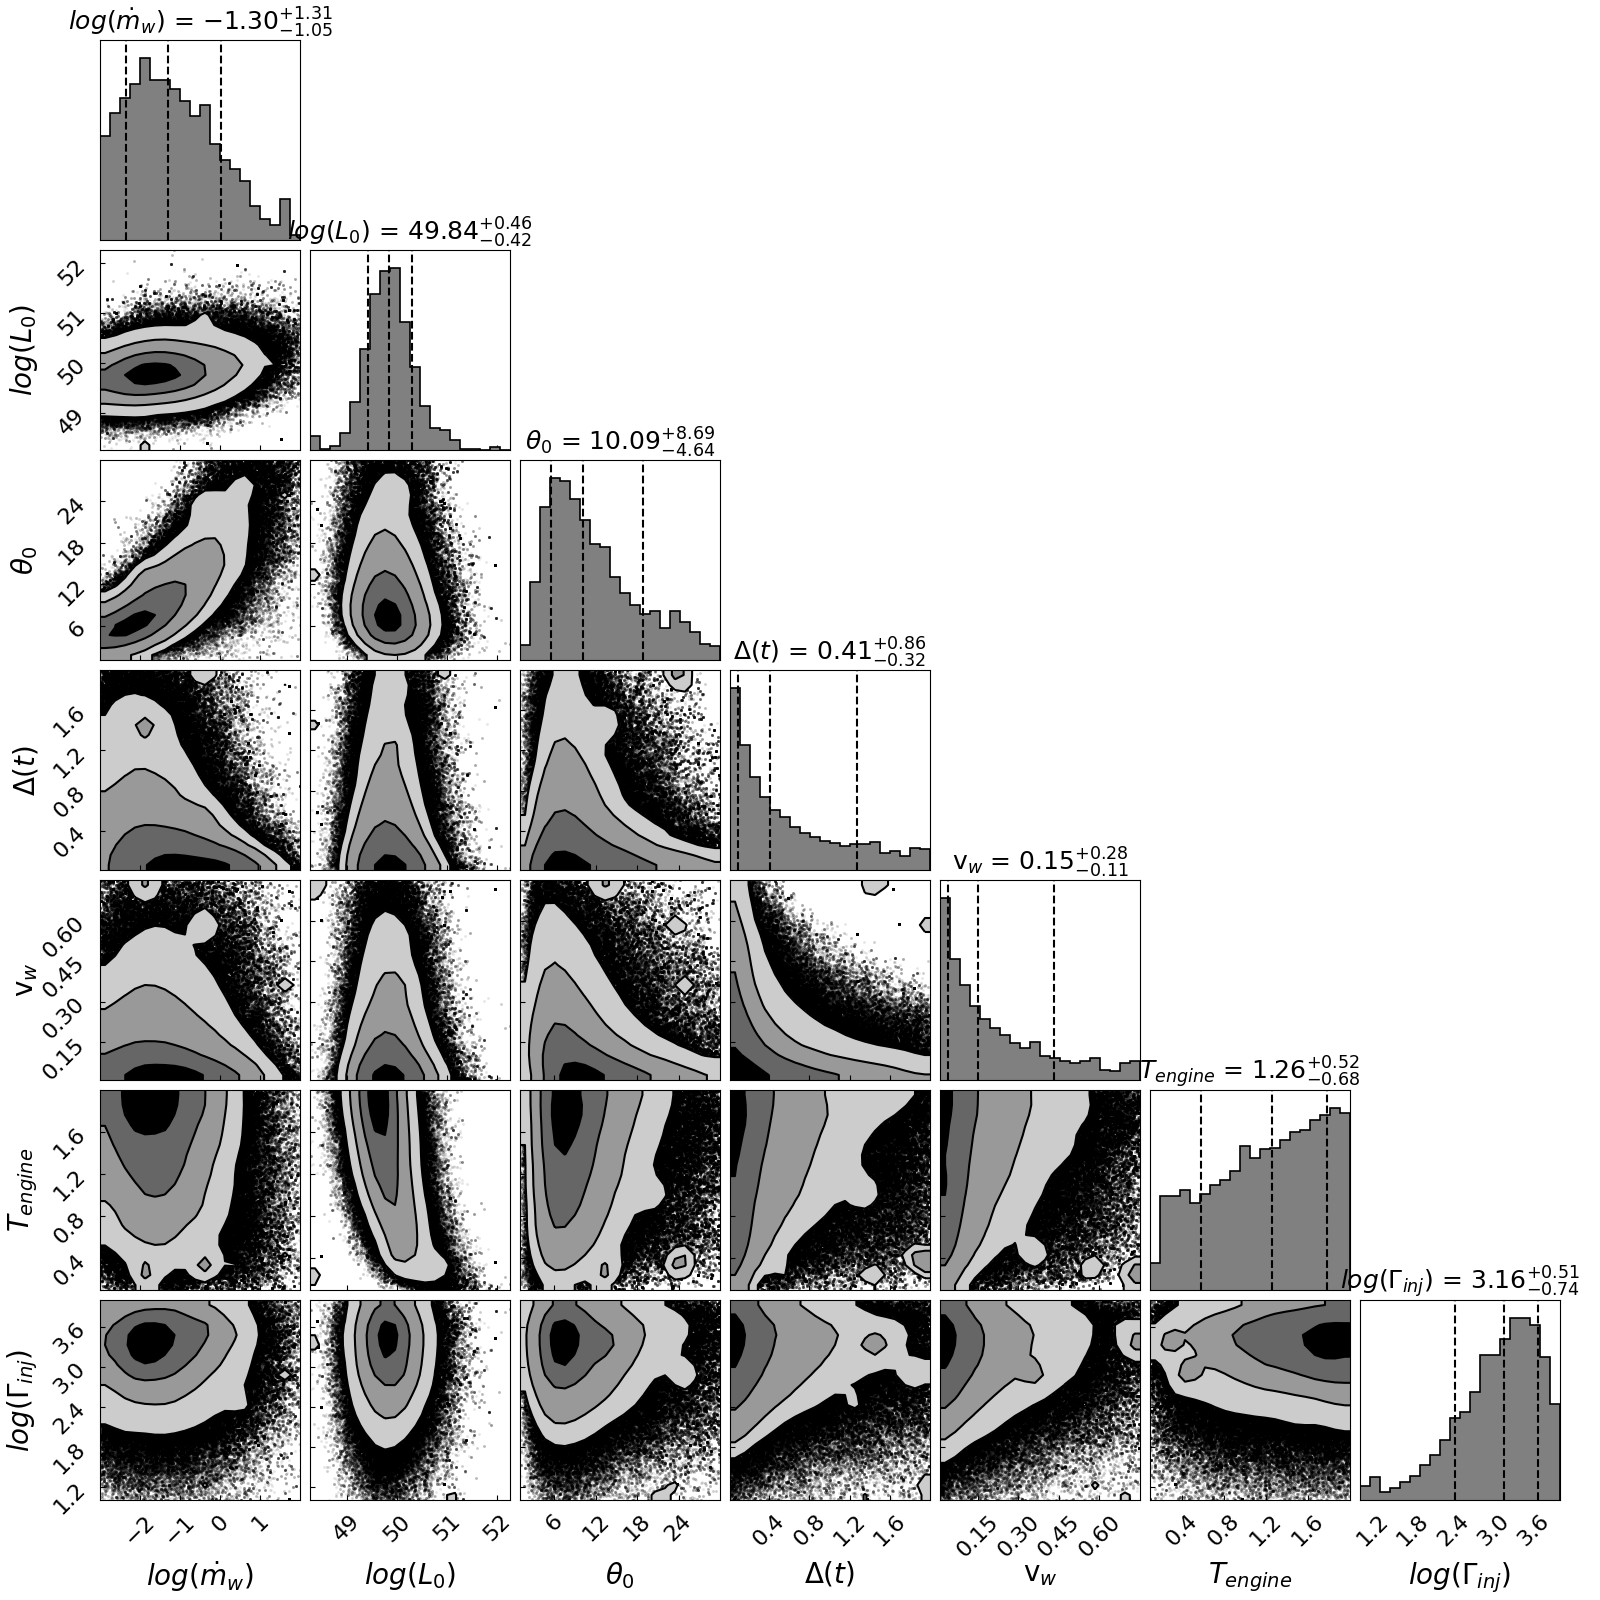
\includegraphics[width=14cm]{images/ch5/mcmc_outflow.png}
	\caption{\fontfamily{lmss}\selectfont Preliminary posterior distributions obtained from our outflow model by applying constraints from a subset of structured jet parameters obtained from the afterglow fits in Table \ref{table:emcee-AG best values}. The histograms in the diagonal of the corner plots show the marginalized posteriors and the inner triangle shows the posterior probabilities. The dashed lines indicate the $16^{\mathrm{th}}$, $50^{\mathrm{th}}$, and $84^{\mathrm{th}}$ quantiles respectively.}
	\label{fig:emcee-outflow}
	\end{center}
\end{figure}

\pagebreak[4]

\clearpage

\begin{table}[htbp!]
\caption{\fontfamily{lmss}\selectfont Bayesian parameter estimation results using our outflow model.}
% \tablefootnote{some kind of footnote from a table, which doesn't work without the tablefootnote package}
\centering
\begin{tabular}{cccc}
\hline\hline
%  & & &  \\
\textbf{Prior bounds} & \textbf{{\fontfamily{qcr}\selectfont emcee} estimate} & \textbf{Units} & \textbf{Description} \\
\hline
\\
$-3 \leq \mathrm{log}(\dot m_w) \leq 2$ & $-1.30^{+1.32}_{-1.05}$ &  \(M_\odot\) /s & rate of mass loss \\
\\
\hline 
\\
$0.01\leq v_w \leq 0.75 $ & $0.15^{+0.28}_{-0.11}$ & c &  wind velocity  \\
\\
\hline 
\\
$1 \leq \theta_0 \leq 30$ & $10.09^{+8.76}_{-4.66}$ & deg & jet angle at injection \\
\\
\hline 
\\
$1\leq \mathrm{log}(\Gamma_{inj}) \leq 4$ & $3.16^{+0.51}_{-0.75}$ & -- & jet Lorentz factor at injection \\
\\
\hline 
\\
$0.01 \leq \Delta t \leq 2$ & $0.41^{+0.87}_{-0.32}$ & s & time delay to jet launch \\
\\
\hline 
\\
$48 \leq \mathrm{log}(L_0) \leq 53$ & $49.85^{+0.46}_{-0.42}$ & erg/s & jet luminosity at injection \\ 
\\
\hline 
\\
$0.1 \leq T_{engine} \leq 2$ & $1.26^{+0.52}_{-0.68}$ & s & activity time of central engine \\ [1ex]
\hline
\hline
\end{tabular}
\label{table:emcee-outflow best values}
\end{table}

\clearpage
\section{Discussion}
\label{ch:Results sec:Discussion}

By performing Bayesian analysis on properties of the structured jet launched by GW170817 using observations of its afterglow, we were able to obtain constraints of some of its key parameters. Using a subset of these parameters, we carried out a second Bayesian analysis to constrain parameters we cannot measure directly---namely properties of the central engine, the jet at injection (i.e., before it propagated into its circumburst environment), and the neutron star ejecta. 

\textit{Central jet engine.–} We found the time delay to jet launch was constrained to be around $\Delta t < 0.41 \ \mathrm{s}$, which is broader than the estimate found by Lazzati and his colleagues ($< 0.36 \ \mathrm{s}$; 2020), and lends credence to the idea that the $\sim$ 1.74 s delay between the GW and $\gamma$-ray detections was likely due to the time it took the jet to propagate through the dense (opaque) NS debris. This also shows that an afterglow model is capable of placing meaningful constraints on properties we are not able to directly measure from the afterglow. While we were not able to place an upper limit on the engine duration time, our best fit value of $T_{engine} = 1.26^{+0.52}_{-0.68} \ \mathrm{s}$. With $T_{engine} < T_{90}$ (recall that $T_{90} < 2 \ \mathrm{s}$ is the divider between long and short GRBs), this supports the idea that neutron star mergers are progenitors of SGRBs.

\textit{Neutron star ejecta.–} The consideration of wind interactions (for both long and short GRBs) is an important departure from the standard model developed in Chapter \ref{ch:Astro theory ssec:GRB AG}, in which we assume a fireball of constant energy expands into an environment of constant density. Our observational evidence of ejecta resulting from GW170817 implies that the relativistic jet must have propagated through that ejecta; and the constraints made on the mass loss rate $\dot m_w$ and velocity $v_w$ of the non-relativistic wind can be used to place constraints on the density of the NS material through the relation,

\begin{equation}
    \rho_w = \frac{\dot m_w}{\Omega_w r^2 v_w},
\end{equation}

assuming spherical symmetry within the solid angle $\Omega_w$ (Lazzati and Perna 2019). The large, positive covariance found between the mass loss rate and jet angle at injection (Fig. \ref{fig:emcee-outflow}) implies that the larger the density of the ejecta material, the broader the jet has to be in order to generate an outflow with properties similar to what we observe.

\textit{Structured jet.–} The injected top-hat jet opening angle was constrained to be around $\theta_{0} = 10.09^{+8.76}_{-4.66} \ \mathrm{degrees}$, which is in agreement (within the errors) with Lazzati and Perna (2019), who made the first measurement of this angle $\theta_{0} = 17.9^{+12.6}_{-3.2} \ \mathrm{degrees}$. After interacting with its environment, the jet-cocoon structure that formed resulted in a brightening of the flux observed in the afterglow at late times. Using radio, optical, and X-ray observations of the afterglow, we were able to constrain the opening angle of the jet core to $\theta_j = 2.15^{+0.80}_{-0.58} \ \mathrm{degrees}$, and the opening angle of the cocoon to $\theta_c = 14.57^{+7.24}_{-7.04} \ \mathrm{degrees}$; however, our analysis of the afterglow model provided a better fit for the jet and the cocoon angle showed degeneracy (i.e., multiple local maxima) when correlated with other parameters, namely the observer angle and jet angle (see Fig. \ref{fig:emcee-JB}). This tells us that different combinations of values for these angles give us similar model flux outputs. We also see a strong positive correlation between the observer and jet angles i.e., a larger inclination requires a larger jet angle to produce the observed fluxes. Besides a jet-cocoon structure geometry that is physically consistent, our results show the jet core to be more energetic than the cocoon---which we would also expect.


%---------------------6.Conclusion------------------------------

\chapter{Conclusion} 
\label{ch:Conclusion}
\begin{fquote}[Toni Morrison][Wellesley College commencement address (2004)] ...contrary to what you may have heard or learned, the past is not done and it is not over, it’s still in process, which is another way of saying that when it’s critiqued, analyzed, it yields new information about itself.
\end{fquote}


The discovery of GW170817, now almost 4 years old, has provided us with the first evidence of binary neutron star mergers, as well as evidence of their principle role in r-process nucleosynthesis. The joint GW-EM detection enabled us to observe the event from inspiral to an afterglow that may continue for years to come, and these observations provided us with a wealth of information and has helped us to improve our theoretical understanding of short gamma-ray bursts and neutron star mergers---a phenomenon first theorized nearly half a century ago. Future joint detections can help us to detect SGRB sources that would otherwise be too faint to detect using $\gamma$-rays alone (e.g., those that may occur in ultra-faint dwarf galaxies; Beniamini et al. 2018), however GW170817 currently stands as the only detection of its kind. 

In this work, we have presented a Bayesian framework and explored the potential of this approach for parameter estimation of the afterglow associated with GW170817, in order to constrain a large range of key observer, jet, neutron star ejecta, and environment parameters. We focused on the GRB afterglow, as opposed to the kilonova or gravitational radiation, because we know that the afterglow lightcurve encodes information such as the jet geometry, the amount of ejecta present, and wind interactions. We performed two parameter estimation analyses using the open-source {\fontfamily{qcr}\selectfont emcee} Python module and showed that results from an afterglow model could be used in a separate study using a semi-analytic jet-cocoon outflow model focused on a set of parameters that cannot be directly observed. In total, we aimed to constrain values for a total of 17 parameters (refer to Tables \ref{table:emcee-AG best values} and \ref{table:emcee-outflow best values} for a list of best fit values). We summarize the main findings below: 

\begin{enumerate}
    \item \textbf{We can obtain constraints on the geometry and energy of a structured jet.} By outfitting our numerical model with a structured jet profile, our Bayesian parameter estimation analysis was able to constrain values for features of the jet-cocoon structure, namely the opening angle of the jet $\theta_j$ and the energies of both the jet and cocoon $E_j$ and $E_c$. In addition, our analysis provides estimates for the parameters that describe the microphysics of the jet's external shocks $\epsilon_e$, $\epsilon_B$, and $p_{index}$, as well as the observer angle $\theta_{obs}$, that are consistent with those found in the literature.

    \item \textbf{We can place constraints on unobservable BNS merger properties.} Using properties of the jet obtained from analysis of the afterglow, we could establish upper limits on wind velocity $v_w$ and the time it took to launch the relativistic jet $\Delta t$. Additionally, we were able to constrain three key properties of the jet at injection---its luminosity $L_0$, its opening angle $\theta_0$, and lower limits on the terminal Lorentz factor $\Gamma_{inj}$.

    \item \textbf{A more robust mulitband observational dataset may help to break parameter degeneracies in our afterglow model.} Many of the bands used from our observational dataset were sparse, with datapoints ranging from 4 (Radio at 1 and 1.5 GHz) to 20 (X-ray band), and bands we did not include contained either one or two points. 
\end{enumerate}

One of the implications of both (1) and (2) is that, rather than engineering one piece of complex software that handles all of the physics, we can employ a piecewise approach in which different pieces of the puzzle are developed, improved on incrementally, and incorporated. Likewise, (2) implies that we can span larger parameter spaces by breaking up our analysis into batches. 

\section{Opportunities for future work}
\label{ch:Conclusion sec:future}

\textit{Assumptions and effects.–} Optimizing the performance of numerical models with accurate physics is a difficult task. There were a number of effects that weren't taken into account in the models we used---for example: a time-varying wind (our model assumed a fixed value), a long-lived central engine (which could have implications for the neutron star ejecta and as a result the afterglow), and geometric asymmetries (we assumed spherical symmetry). One thing we were unable to thoroughly test given time constrains was our afterglow model's sensitivity to different ranges of priors. Future work could include:
\begin{itemize}
    \item Comparing the results of two or more afterglow models (e.g., utilizing the afterglow code developed by Morsony et al. 2016).
    \item Conducting a robust test of model sensitivity to priors.
    \item Spanning a larger parameter space (e.g., probing tidal deformability). 
    \item Incorporating machine learning algorithms and or high-performance computing techniques to improve the time it takes to perform Bayesian analysis on resource-intensive numerical models.
    \item Performing the analysis presented in this work on a larger set of observed SGRB afterglows. 
\end{itemize}

\textit{The search continues.–}Just as we enumerated the questions that motivated this work at the beginning of this thesis, we close with a list of general questions motivated both by our results and the current state of research into GW170817:

\begin{itemize}
    \item What implications, if any, would our estimate for the time delay to jet launch have for estimations of how long it took GW170817 to collapse into a black hole (estimated to be $\sim 1 \ \mathrm{s}$; e.g., Gill et al. 2019)?
    \item What could the most recent observations of GW170817's afterglow reveal about the nature of its central engine?
    \item How would a more robust observational dataset of GW170817's afterglow have impacted the outcome of this analysis?
    \item Are there parameter estimates that could be improved with the addition of multimessenger (i.e., gravitational wave) data?
    \item How would our current understanding of BNS mergers change with observational data of other merger events? In particular, how would using the methods we have employed improve our parameter estimates for properties of the structured jet and merger remnant?
\end{itemize}

\section{Data availability}
\label{ch:Conclusion sec:source code}


While the models used in this work are proprietary, the observational dataset and cleaning data script, as well as the scripts used to generate {\fontfamily{qcr}\selectfont emcee} fits can be found on the author's GitHub space-isa/Parameter-estimation-GW170817 at \href{http://doi.org/10.5281/zenodo.4609341}{http://doi.org/10.5281/zenodo.4609341} (Rodriguez 2021). We highly encourage users to fork this repo and develop it to fit their project's needs. Users looking to utilize {\fontfamily{qcr}\selectfont emcee} for their afterglow models, for example, can provide their numerical model, define a set of free parameters of interest, and adjust sampler parameters as needed.


% \appendix
% \chapter{Data cleaning script}

% \textbf{Code Example:}
% \begin{minted}[bgcolor=bg,
%               frame=lines,
%               framesep=2mm]{python}
%     #!/usr/bin/env python2

%     def example_function():
%         return "hello world"

%     a = 5
%     b = "I am python code"
% \end{minted}

% \chapter{Emcee-outflow code}

% \textbf{Code Example:}
% \begin{minted}[bgcolor=bg,
%               frame=lines,
%               framesep=2mm]{python}
%     #!/usr/bin/env python2

%     def example_function():
%         return "hello world"

%     a = 5
%     b = "I am python code"
% \end{minted}

% \chapter{Structured jet profile code}

\pagebreak

\backmatter
\renewcommand{\chaptermark}[1]{\markboth{\textsc{#1}}{}} %<---------
                           %THIS MAKES THE \leftmark FORMAT WITH
                           %SMALLCAPS & NO CHAPTER NUMBERING
                           %AND WILL BE USED FOR ALL BACK MATTER
                           
\chapter{Afterword}
\begin{fquote}[Audre Lorde][The Berlin Years][] I believe in societies that do not use members of that society for the profit of other parts of that society. I believe passionately in societies that define the good in terms of human needs as opposed to terms of profit. I believe that it is possible to have societies that don't categorize, reject, trivialize, objectify, other human beings because of their differences. That we can be different and use those differences not to destroy each other, but to move. These are the things I believe, and everything I breathe, say, and do is a part of that---the way I eat, the way I raise my children, the way I teach, the way I write, and it gives me joy in the doing.
\end{fquote}

This thesis was written in the midst of a deadly global pandemic---one that has resulted so far in over two million deaths worldwide, with nearly a quarter of those deaths in the US---and on the heels of a global uprising for Black lives and the abolition of the prison industrial complex sparked by the murder of George Floyd by the police state. In the ``great awakening" that followed, Black people across the country were asked, by those considered by Dr. Martin Luther King Jr. to be the greatest stumbling block in the stride towards freedom, if we thought this moment would be the one that would finally bring change. History has shown us that Black strides tend to be met with white rage\footnote{\fontfamily{lmss}\selectfont Anderson, C. (2016). White rage: The unspoken truth of our racial divide. Bloomsbury Publishing USA.}, Black resistance with violence and the cooptation of movement and language. Sure enough, TIME magazine would rename the uprisings of Summer 2020 into the ``Racial Justice Movement", use a picture of Floyd as its face, and nominate it as a one of their finalists for their 2020 Person of the Year. A nameless Black face. An attempt to defang a movement that declared “All Black lives matter.” Violent erasure, unfolding now as it has time and time again.

Through all of this, our work didn't stop. Not for the pandemic, (though tens of millions in the US became unemployed and were pushed into houselessness because our government values profits over people), not for the uprisings, not for the collective trauma resulting from Black death put on public display for weeks on end, and not for the acts of domestic terrorism that came to a head with a failed coup attempt. Universities did not extend trauma-informed leadership to their faculty and staff, nor did they expect it of them---even though the mental health impacts on Black Americans following police killings are measurable\footnote{\fontfamily{lmss}\selectfont Bor, J., Venkataramani, A.S., Williams, D.R., and Tsai, A.C. (2018). Police killings and their spillover effects on the mental health of black Americans: a population-based, quasi-experimental study. The Lancet, 392(10144), 302-310.}, even after students across the country rallied together to make themselves heard in protest. Oregon State University College of Science students would learn that their efforts to disrupt the status quo were simply one in a long cycle going back decades: student agitation turned into listening sessions, turned into under-resourced committees---with permutations of D, E, and I (and sometimes, J and C)---turned into new offices and programs, diversity statements, strategic plans, initiatives.  

But what are diversity initiatives to a Black scholar? It brings to mind the question asked of W.E.B. DuBois over a century ago, though never directly, “How does it feel to be a problem?”\footnote{\fontfamily{lmss}\selectfont Du Bois, W.E.B. (1982). The souls of black folk (p.43). Penguin Books Ltd.}. At that time it was the color-line problem, before then the slave problem, later the civil rights problem, today the diversity problem---and tomorrow? So long as white supremacy has its hold at the root, tomorrow we will be viewed as a problem still. Within academic institutions, as Dr. Tao Leigh Goffe, assistant professor of literary theory and cultural history at Cornell University states, \textit{``diversity is a white supremacy solution to a white supremacy problem"}\footnote{\fontfamily{lmss}\selectfont Goffe, T.L. [@taoleighgoffe]. (2020, Nov. 25). ‘diversity’ is a white supremacist answer to a white supremacist problem [Tweet]. Twitter. https://twitter.com/taoleighgoffe/status/1331739382768951297}. Academic institutions are places in which we as people from marginalized communities are collapsed into passive acronyms (see: URM), while simultaneously being used as selling points to prospective (white) students and their families; and where victims of violent institutional structures are considered legal liabilities to be handled with the utmost care. Intersectionality is erased through aggregated data or through claims of not having enough data points. When it’s not erased it becomes a hyperfocus---the “firsts” discovered in archives, the “onlies” who are used in advertisements, brought to the front and center of lab photos, who are asked to freely extend, then overextend, their emotional and intellectual labor in service of ``diversity”. As Dr. Angela Y. Davis shared in her 2019 lecture ``Freedom is a Constant Struggle,"\footnote{\fontfamily{lmss}\selectfont Delivered at an the international seminar “Democracia em colapso?”, in S\~{a}o Paulo, Brazil.} \textit{``We always seem prime to celebrate individual advancements: individual advancements of Black people, of people of color, of women, without taking into consideration that diversity by itself may simply mean that previously marginalized individuals have been recruited to guarantee a more efficient operation of oppressive systems...What is the point of endorsing race and gender diversity within a framework that remains heteropatriarchal at its core?"}. 

Meanwhile, change really means slowly draining resources (defunding) programs created to provide structural student support services, in addition to defunding cultural centers and departments dedicated to the study of race(ism), ethnicity, Indigeneity, gender and sexuality. It means unveiling a new name for the annual rival football game, or announcing that an anonymous donation will be used to fund a stadium instead of prioritizing the material needs of the students (which includes student athletes), faculty, instructors, and staff that have been impacted by the pandemic and its economic fallout. It means redirecting Black curiosity in the classroom or in the advising office. Changing the face of on-campus policing. Change only to maintain law and order (read: comfort).

In the sciences, that order is white empiricism (Prescod-Weinstein, 2020) which makes it  difficult for those who embody ``otherness" to persist as scientists. The current underrepresentation of Black, Indigenous women and non-binary people of color stems from a history of exclusion and is a symptom of STEM culture---and many who have left \textit{``often report a sense of loneliness, discrimination and rejection as it relate[ed] to moving through their STEM trajectories"} (Isler et al. 2020, p.3). The history of scientific discoveries show that physicists and astronomers will persist for decades and move mountains (sometimes literally) to revolutionize their fields. And what could be more revolutionary than for scientific communities to be as committed to transformative social and cultural change as they are to pushing the boundaries of knowledge? Dismantling systems of oppression, like learning and research, is hard, life-long work. It will require you to sit in your discomfort, to be inconvenienced, to critically examine your philosophies, ideologies and practices, to make sacrifices, decline opportunities, and take risks. There is no need to start from scratch, nor do we need any more one-off task forces comprised of well-intentioned but over-committed and inexperienced members, or siloed committees created to ``bear the DEI burden" of their departments. There is a wealth of information and expertise (past and present) that can and should be accessed if STEM institutions are truly invested in transformative change: changes to policies and procedures that keep the most marginalized and vulnerable communities at the center, as well as changes to institutional and workplace culture from one that values competition, gatekeeping, and overwork to one that values empathy, equity, and care.  

\pagebreak

\bibliography{thesis}
\bibliographystyle{apacite}
\nocite{*}

\end{document}